\documentclass[11pt]{article}

\usepackage[margin=1in]{geometry}

\usepackage{amsmath, amsthm, amssymb, microtype, enumerate, stackrel, mathrsfs, tikz}
\usepackage[colorlinks, citecolor=blue, linkcolor=blue, bookmarks=true]{hyperref}
\usepackage[nameinlink, noabbrev, capitalize]{cleveref}

\usepackage{bbm}
\usepackage{ulem} 

\usepackage{cleveref}
\usepackage[ruled,vlined]{algorithm2e}


\usepackage{float}
\usetikzlibrary{positioning}

\def\E{\mathbb{E}}
\def\P{\mathbb{P}}


\def\BAD{\mathrm{BAD}}
\def\BLK{\mathrm{BLK}}
\def\REP{REP}
\def\SOM{SOM}
\def\CON{\mathrm{CON}}
\def\SourceDomain{\mathsf{SourceDomain}}
\def\CoDomain{\mathsf{CoDomain}}
\def\Supp{\mathsf{Supp}}
\def\BAD{\mathrm{BAD}}
\def\BLK{\mathrm{BLK}}
\def\REP{\mathrm{REP}}
\def\SOM{\mathrm{SOM}}
\def\CON{\mathrm{CON}}
\def\SourceDomain{\mathrm{SourceDomain}}
\def\CoDomain{\mathrm{CoDomain}}
\def\Supp{\mathrm{Supp}}


\newcommand{\func}[1]{\mathrm{#1}}
\newcommand{\funcfamily}[1]{\mathcal{#1}}
\newcommand{\tensor}[1]{\mathfrak{#1}}
\newcommand{\randtensor}[1]{\mathbf{#1}}


\newcommand{\Cond}{\mathrm{Cond}}
\newcommand{\Merge}{\mathrm{Merge}}
\newcommand{\Disp}{\mathrm{Disp}}
\newcommand{\INW}{\mathsf{INW}}



\newtheorem{lemma}{Lemma}[section]
\newtheorem{theorem}[lemma]{Theorem}
\newtheorem{proposition}[lemma]{Proposition}
\newtheorem{corollary}[lemma]{Corollary}
\newtheorem{definition}[lemma]{Definition}
\newtheorem{claim}[lemma]{Claim}
\newtheorem{observation}[lemma]{Observation}
\newtheorem{assumption}[lemma]{Assumption}
\newtheorem{fact}[lemma]{Fact}
\newtheorem*{remark}{Remark}
\newtheorem{summary}[lemma]{Summary}

\newcommand{\R}{\mathbb{R}}
\newcommand{\Q}{\mathbb{Q}}
\newcommand{\N}{\mathbb{N}}
\newcommand{\Z}{\mathbb{Z}}
\newcommand{\C}{\mathbb{C}}
\newcommand{\F}{\mathbb{F}}
\newcommand{\vstart}{v_{\normalfont\text{start}}}
\newcommand{\vacc}{v_{\normalfont\text{acc}}}
\newcommand{\eps}{\varepsilon}


\newcommand{\AC}{\mathrm{AC}}
\newcommand{\NC}{\mathrm{NC}}
\newcommand{\Ext}{\mathrm{E\textsc{xt}}}
\newcommand{\depth}{\mathrm{Depth}}
\newcommand{\Samp}{\mathrm{Samp}}
\newcommand{\SD}{\mathrm{SD}}

\newcommand{\Rot}{\mathsf{Rot}}
\newcommand{\Spc}{\mathsf{Spc}}


\newcommand{\TC}{\mathsf{TC}}

\newcommand{\NZ}{\mathsf{NZ}}
\newcommand{\PRG}{\mathsf{PRG}}
\newcommand{\WPRG}{\mathsf{WPRG}}



\DeclareMathOperator{\poly}{\mathrm{poly}}
\DeclareMathOperator{\supp}{\mathrm{Supp}}
\DeclareMathOperator{\polylog}{\mathrm{polylog}}
\DeclareMathOperator{\layer}{layer}


\newcommand{\sv}{\overset{sv}{\approx}}
\newcommand{\ds}{\textcircled{p}}
\newcommand{\WE}{\widetilde{\mathbb{E}}}

\newcommand{\reduct}[1]{\mathsf{#1}}


\begin{document}


\title{
Weighted Pseudorandom Generators for Read-Once Branching Programs via Weighted Pseudorandom Reductions
}

\author{ 
Kuan Cheng \footnote{CFCS, School of Computer Science, Peking University. ckkcdh@pku.edu.cn.}
\and 
Ruiyang Wu \footnote{CFCS, School of Computer Science, Peking University. wuruiyang@stu.pku.edu.cn.}
}

\date{}
\maketitle


\begin{abstract}

    We study weighted pseudorandom generators (WPRGs) and derandomizations for read-once branching programs (ROBPs), which are key problems towards answering the fundamental open question $\mathbf{BPL}  \stackrel{?}{=} \mathbf{L}$.
    Denote $n$ and $w$ as the length and the width of a ROBP.
    We have the following results.
    
    For standard ROBPs, there exists an explicit $\varepsilon$-WPRG with seed length
        $$  O\left(\frac{\log n\log (nw)}{\max\left\{1,\log\log w-\log\log n\right\}}+\log w \left(\log\log\log w-\log\log\max\left\{2,\frac{\log w}{\log n/\varepsilon}\right\}\right)+\log(1/\varepsilon)\right).$$
    When $n = w^{o(1)}$, this is better than the constructions in \cite{hozaBetterPseudodistributionsDerandomization2021, cohenErrorReductionWeighted2021, pynePseudodistributionsThatBeat2021, chattopadhyayOptimalErrorPseudodistributions2020}.
    
    For permutation ROBPs with unbounded widths and single accept nodes, there exists an explicit $\varepsilon$-WPRG with seed length
        $$     O\left( \log n\left( \log\log n + \sqrt{\log(1/\varepsilon)} \right)+\log(1/\varepsilon)\right). $$
    This slightly improves the result of \cite{chenWeightedPseudorandomGenerators2023}.
    
    For regular ROBPs with $n \le 2^{O(\sqrt{\log w})}, \varepsilon = 1/\poly w$, we give a derandomization within space $O(\log w)$, i.e. in $\mathbf{L}$ exactly.
    
    This is better than previous results of \cite{ahmadinejadHighprecisionEstimationRandom2022, chenWeightedPseudorandomGenerators2023, chattopadhyayRecursiveErrorReduction2023} in this regime.
    
    Our main method is based on a recursive application of weighted pseudorandom reductions, which is a natural notion that is used to simplify ROBPs.
    
    
        
\end{abstract}


\section{Introduction}

Randomness is a fundamental resource in computation, but is it essential? A key conjecture in space-bounded computation is that randomized algorithms in the complexity class $\mathbf{BPL}$ can be efficiently simulated by deterministic logspace algorithms, i.e. $\mathbf{BPL}=\mathbf{L}$. A central approach toward addressing this conjecture is the derandomization of standard-order read-once branching programs (ROBPs), which is usually defined as the following.

\begin{definition}[Read-once branching programs (ROBP)]
    A read-once branching program $f$ of length $n$, width $w$ and alphabet size $|\Sigma|=2^s$ is a directed acyclic graph with $n+1$ layers $V_0,\ldots,V_n$. For any layer $V_i$ except $V_n$, each node $v\in V_i$ has $2^s$ outgoing edges to nodes in $V_{ i+1}$. These edges are labeled by distinct symbols in $\Sigma$. There exists a unique start node $v_{start} \in V_0$ and a set of accept nodes $V_{accept}\subset V_n$. Given an input $x\in \Sigma^n$, the computation of $f(x)$ is defined as: 
    $f(x) = 1$, if there exists a unique path $v_{start},v_1,\ldots,v_n$ such that the edge between $v_i$ and $v_{i+1}$ is labeled by $x_i$, and $v_n\in V_{accept}$;  $f(x) = 0$ otherwise.
\end{definition}
Every problem in $\mathbf{BPL}$ can be reduced to approximating $\mathbb{E}f$ for a corresponding ROBP $f$. A classical method for derandomizing ROBPs is constructing pseudorandom generators (PRGs).

\begin{definition}[PRG]
    Let $\mathcal{F}$ be a class of ROBPs $f:(\{0,1\}^s)^n\to \{0,1\}$.
    An $\varepsilon$-PRG for $\mathcal{F}$ is a function  $G:\{0,1\}^d\to (\{0,1\}^s)^n$
    such that for every $f\in \mathcal{F}$, we have
    \begin{equation*}
        \left|\E_{x\in (\{0,1\}^s)^n}f(x)-\E_{r\in \{0,1\}^d}f(G(r))\right|\leq \varepsilon.
    \end{equation*}
    The input length $d$ is called the seed length of the PRG. We say that $G$ is \textbf{explicit} if it can be computed in space $O(d)$ and time $\poly(d, n)$.


\end{definition}


Using the probabilistic method, one can show the existence of a non-uniform $\varepsilon$-PRG for standard-order ROBPs of length $n$, width $w$, and alphabet size $2^s$, with an optimal seed length of $O(s+\log(nw/\varepsilon))$. 
However, constructing explicit PRGs that have short seed lengths turns out to be an exceptional challenge. In a seminal work, Nisan \cite{nisanPseudorandomGeneratorsSpacebounded1992} constructed an explicit $\varepsilon$-PRG for ROBPs of length $n$, width $w$, and binary alphabet $\{0,1\}$, with a seed length of $O(\log n\log(nw/\varepsilon))$. Building on this result, Saks and Zhou \cite{saksBPHSPACEDSPACES31999} developed a celebrating algorithm to derandomize $\mathbf{BPL}$, within $O(\log^{3/2}n)$ space deterministically.
Nisan \cite{nisan1992rl} also used \cite{nisanPseudorandomGeneratorsSpacebounded1992} to show that $\mathbf{BPL \subseteq \mathbf{SC}}$.
Impagliazzo, Nisan, and Wigderson \cite{impagliazzoPseudorandomnessNetworkAlgorithms1994} generalized the construction of \cite{nisanPseudorandomGeneratorsSpacebounded1992} by using expanders, to fool more general models in network communication.
In the meantime, for short ROBPs, Nisan and Zuckerman \cite{nisanRandomnessLinearSpace1996} gave another remarkable PRG that has a better seed length for wide but short ROBPs, i.e. with seed length $O(\log w)$ when $n = \poly \log w, \eps = 2^{-\log^{0.99} w}$.
Armoni \cite{armoniDerandomizationSpaceBoundedComputations1998}  further extended \cite{nisanPseudorandomGeneratorsSpacebounded1992, nisanRandomnessLinearSpace1996} to construct an improved PRG with seed length\footnote{\cite{armoniDerandomizationSpaceBoundedComputations1998} needs to use an extractor with seed length optimal up to constant factors which is discovered later than \cite{armoniDerandomizationSpaceBoundedComputations1998}, e.g. \cite{guruswamiUnbalancedExpandersRandomness2009}.
} $O\left(\frac{\log n\log (nw/\varepsilon)}{\max\{1, \log\log w-\log\log (n/\varepsilon)\}} \right)$.

\subsection{Weighted Pseudorandom Generators}

Despite years of research, the challenging problem of constructing better PRGs for general ROBPs remains open. Nisan's generator is still the best explicit PRG for ROBPs when lengths and widths are large, e.g. $n= w= 1/\varepsilon$. However, PRGs are not the only black-box solution to derandomization. 
Weighted pseudorandom generator (WPRG) and Hitting set generator (HSG) can also do derandomizations.

Braverman, Cohen, and Garg \cite{braverman2019pseudorandom} introduced WPRG which is a weaker notion than PRG.
\begin{definition}[WPRG]
    Let $\mathcal{F}$ be a class of ROBPs $f:(\{0,1\}^s)^n\to \{0,1\}$. A $W$-bounded $\varepsilon$-WPRG for $\mathcal{F}$ is a function $(G,w):\{0,1\}^d\to(\{0,1\}^s)^n\times \mathbb{R}$ such that for every $f\in \mathcal{F}$, we have
    \begin{align*}
        &\left|\E_{x\in(\{0,1\}^s)^n}f(x)-\sum_{r\in \{0,1\}^d}\left[\frac{1}{2^d}w(r)\cdot  f(G(r))\right]\right|\leq \varepsilon,\\
        &\forall r, |w(r)|\leq W.
    \end{align*}
    The input length $d$ is called the seed length of the WPRG. We say that $(G,w)$ is \textbf{explicit} if it can be computed in space $O(d)$.
\end{definition}
As shown in \cite{braverman2019pseudorandom}, under this notion, the seed length can be better than those of previous PRGs in the sense that for $\varepsilon$ there is only an isolated addend in the seed length.
Chattopadhyay and Liao \cite{chattopadhyayOptimalErrorPseudodistributions2020} further improved this isolated addend to be optimal $O(\log (1/\varepsilon))$.
Meanwhile, Ahmadinejad, Kelner, Murtagh, Peebles, Sidford, and Salil Vadhan \cite{ahmadinejadHighprecisionEstimationRandom2022} developed another method based on Richardson Iterations to reduce errors in derandomizing random walks for certain specific graphs.
Then Cohen, Doron, Renard, Renard, Sberlo, and Ta-Shma \cite{cohenErrorReductionWeighted2021}, and also Pyne and Vadhan \cite{pynePseudodistributionsThatBeat2021} further developed this technique to be a black-box error reduction from PRGs to WPRGs.
Hoza \cite{hozaBetterPseudodistributionsDerandomization2021} improved this construction to attain seed length $O(\log n \log (nw) + \log (1/\varepsilon))$ for the binary alphabet.

Inspired by error reductions used in these WPRG constructions, Hoza \cite{hozaBetterPseudodistributionsDerandomization2021} improved the deranomization of Saks and Zhou \cite{saksBPHSPACEDSPACES31999} to be $\mathbf{BPL}\subseteq \mathbf{DSPACE}\left(\frac{\log^{3/2}n}{\sqrt{\log\log n}}\right)$. 
Cohen, Doron, Sberlo, and Ta-Shma \cite{cohenApproximatingIteratedMultiplication2023}, also Pyne and Putterman \cite{puttermanOptimalDerandomizationMediumWidth2022},  showed that ROBPs with medium width $w = 2^{O(\sqrt{\log n})}$ can be drandomized in $\tilde{O}(\log n)$ space.
Cheng and Wang \cite{cheng2024bpl} showed that $\mathbf{BPL} \subseteq \mbox{logspace-uniform } \mathbf{AC}^1$.


HSG is an even weaker notion than WPRG. However, it is also a powerful tool in derandomization.
\begin{definition}[HSG]
    Let $\mathcal{F}$ be a class of ROBPs $f:(\{0,1\}^s)^n\to \{0,1\}$. An $\varepsilon$-HSG for $\mathcal{F}$ is a function $H:\{0,1\}^d\to (\{0,1\}^s)^n$ such that for every $f\in \mathcal{F}$, if $\E_{x\in (\{0,1\}^s)^n}f(x)\geq \varepsilon$, then $\exists r\in \{0,1\}^d, f(H(r))=1$.

The input length $d$ is called the seed length of the HSG. We say that $H$ is \textbf{explicit} if it can be computed in space $O(d)$.
\end{definition}
One can use HSG to find an accepting path when the acceptance probability is significant.
Actually, HSG is more powerful than this. 
Cheng and Hoza \cite{chengHittingSetsGive2020} showed how to approximate the acceptance probabilities of ROBPs of length $n$, width $w$ using an HSG for ROBPs with significantly larger width $O(\poly(nw/\varepsilon))$ and length $O(\poly(nw/\varepsilon))$. 
Pyne, Raz, and Zhan \cite{pyne2023certified} further extended the method to give a deterministic sampler for such a task.
Constructing better HSGs is a also challenging task. 
Hoza and Zuckerman gave the current best HSG with seed length $O\left( \frac{\log n \log (nw)}{\max\{1, \log\log w- \log \log n\}} + \log(1/\varepsilon) \right)$ for binary alphabet.






\subsection{WPRG for short-wide standard ROBPs}


Although significant progress has been made in the study of WPRGs for general ROBPs with equal length and width, the known WPRGs for the regime of short-wide ROBPs, where $n=\poly(\log w)$, has no advantage compared to early works \cite{nisanPseudorandomGeneratorsSpacebounded1992,impagliazzoPseudorandomnessNetworkAlgorithms1994, nisanRandomnessLinearSpace1996, armoniDerandomizationSpaceBoundedComputations1998}. 
For binary alphabet, NZ PRG \cite{nisanRandomnessLinearSpace1996} and Armoni's PRG \cite{armoniDerandomizationSpaceBoundedComputations1998} have optimal seed lengths of $O(\log w)$ when $\varepsilon=2^{-\log^{1-v}w}$, where $v$ is any constant in $(0,1)$. When we need a smaller error such as $\varepsilon=1/\poly(w)$, the WPRGs by \cite{cohenErrorReductionWeighted2021, hozaBetterPseudodistributionsDerandomization2021, pynePseudodistributionsThatBeat2021} have seed lengths deteriorates to $O(\log w\log\log w)$ which is the same as that of \cite{nisanPseudorandomGeneratorsSpacebounded1992, impagliazzoPseudorandomnessNetworkAlgorithms1994, armoniDerandomizationSpaceBoundedComputations1998}. 
This naturally raises the question: can we construct a WPRG for short-wide ROBPs with seed length $O(\log w+\log(1/\varepsilon))$ for this regime?
The question is also interesting for larger $n$, i.e. can we have a WPRG construction with seed length meeting that of the HSG construction in \cite{hoza2020simple}.

In this paper, we make progress for answering these questions by constructing a $\varepsilon$-WPRG for ROBPs of width $w$ and length $n$ with better seed length. Specifically, we achieve the following results.
\begin{theorem}\label{thm:intro armoni improved} 
    For every $n, w\in \mathbb{N}$, $\varepsilon\in (0,1)$, with $n \ge \log w$, there exists an explicit $\varepsilon$-WPRG 
    with seed length
    \begin{equation*}
        O\left(\frac{\log n\log (nw)}{\max\left\{1,\log\log w-\log\log n\right\}}+\log w \left(\log\log\log w-\log\log\max\left\{2,\frac{\log w}{\log n/\varepsilon}\right\}\right)+\log(1/\varepsilon)\right)
    \end{equation*}
    for the class of ROBPs of width $w$, length $n$ and alphabet $\{0,1\}$.
\end{theorem}
This WPRG has a better seed length than Armoni's PRG \cite{armoniDerandomizationSpaceBoundedComputations1998,kaneRevisitingNormEstimation2009}.
Also, this slightly outperforms \cite{hozaBetterPseudodistributionsDerandomization2021, cohenErrorReductionWeighted2021, pynePseudodistributionsThatBeat2021, chattopadhyayOptimalErrorPseudodistributions2020}, when $  n <<\poly(w)$.

For the special case $n = \poly \log w$, we have the following result.
\begin{theorem}\label{thm:intro nz improved}
    Given any constant $C>0$, for every $w, s\in \mathbb{N}$ and $\varepsilon\in (0,1)$, there exists an explicit $\varepsilon$-WPRG with seed length 
    \begin{equation*}
        O(s+\log w\log\log\log w+\log(1/\varepsilon))
    \end{equation*}
    for the class of ROBPs of width $w$, length $n=\log^{C}w$ and alphabet $\{0,1\}^s$.
\end{theorem}
\cref{tab:nz comparison} and \cref{tab:armoni comparison} summarize the seed length of $\varepsilon$-PRGs, $\varepsilon$-HSGs and $\varepsilon$-WPRGs for short-wide general ROBPs. 

\begin{table}[H]
    \centering
    \begin{tabular}{c|c|c}
        Seed length&Type&Reference\\
        \hline
        $O\left(\frac{\log n\log (nw/\varepsilon)}{\log\log w-\log\log (n/\varepsilon)}\right)$&PRG&\cite{armoniDerandomizationSpaceBoundedComputations1998,kaneRevisitingNormEstimation2009}\\
        $O(\log n\log(nw)+\log(1/\varepsilon))$&WPRG&\cite{hozaBetterPseudodistributionsDerandomization2021}\\
        $O\left(\frac{\log n\log (nw)}{\log\log w-\log\log n}+\log (w/\varepsilon)\log\log_n(1/\varepsilon)\right)$&WPRG&\cite{cohenErrorReductionWeighted2021}\\
        $O\left(\frac{\log n\log (nw)}{\log\log w-\log\log n}+\log (1/\varepsilon)\right)$&HSG&\cite{hoza2020simple}\\
        $O\left(\frac{\log n\log (nw)}{\log\log w-\log\log n}+\log w \log\log\log w+\log(1/\varepsilon)\right)$&WPRG&This work\\
    \end{tabular}
    \caption{Comparison of seed length of $\varepsilon$-PRGs,  $\varepsilon$-HSGs and $\varepsilon$-WPRGs for general ROBPs of width $w$, length $n \le \sqrt{w}$, and alphabet $\{0,1\}$, where $\varepsilon\leq 1/\poly(w)$.}
    \label{tab:armoni comparison}
\end{table}

\begin{table}[H]
    \centering
    \begin{tabular}{c|c|c|c}

        Seed length&Type&Reference&Note\\
        \hline
        $O(\log w)$&PRG&\cite{nisanRandomnessLinearSpace1996}&$\varepsilon=2^{-\log^{1-v}w}$\\
        $O(\log(w/\varepsilon)\log\log w)$&PRG&\cite{nisanRandomnessLinearSpace1996},\cite{impagliazzoPseudorandomnessNetworkAlgorithms1994},\cite{nisanPseudorandomGeneratorsSpacebounded1992}\\
        $O(\log w\log\log w+\log(1/\varepsilon))$&WPRG&\cite{hozaBetterPseudodistributionsDerandomization2021},\cite{cohenErrorReductionWeighted2021}&\\
        $O(\log w+\log(1/\varepsilon))$&HSG&\cite{hoza2020simple}&\\
       
        $O(\log w\log\log\log w+\log(1/\varepsilon))$&WPRG&This work&\\
        \hline
        $O(\log w+\log(1/\varepsilon))$&PRG&folklore& Optimal; non-explicit\\
    \end{tabular}
    \caption{Comparison of seed length of $\varepsilon$-PRGs,  $\varepsilon$-HSGs and  $\varepsilon$-WPRGs for short-wide ROBPs of width $w$, length $n=\poly(\log w)$, and alphabet $\{0,1\}$.}
    \label{tab:nz comparison}
\end{table}







\subsection{WPRG for unbounded-width permutation ROBPs with a single accepting node}
Recently researchers have also spent much effort on derandomization for special classes of ROBPs.
One such class is permutation ROBPs, where the transition functions between layers are permutations.
\begin{definition}[permutation ROBP]
    A (standard-order) permutation ROBP is a standard-order ROBP $f$, where for every $i\in [n]$ and $x\in \{0,1\}^s$, the transition matrix from $V_i$ to $V_{i+1}$ through edges labeled by $x$, is a permutation matrix in $\mathbb{R}^{w\times w}$.
\end{definition}

Early work on PRGs for permutation ROBPs \cite{brody2010coin, de2011pseudorandomness, koucky2011pseudorandom, steinke2012pseudorandomness, reingold2013pseudorandomness, chattopadhyay2019pseudorandom} focus on the constant width case. 
Inspired by the progress on derandomizing squares \cite{rozenmanDerandomizedSquaringGraphs2005,ahmadinejadHighprecisionEstimationRandom2022, ahmadinejad2023singular}, recent studies focus on unbounded-width permutation ROBPs with a single accepting node \cite{hozaPseudorandomGeneratorsUnboundedWidth2020,pynePseudodistributionsThatBeat2021, bogdanov2022hitting,chenWeightedPseudorandomGenerators2023}. 
Hoza, Pyne and Vadhan \cite{hozaPseudorandomGeneratorsUnboundedWidth2020} designed an $\varepsilon$-PRG for unbounded-width permutation ROBPs with seed length $\widetilde{O}(\log n\log(1/\varepsilon))$ for binary alphabet. 
They also proved that any PRG for this class must have seed length $\widetilde{\Omega}(\log n\log(1/\varepsilon))$. 
For the WPRG case, Pyne and Vadhan \cite{pynePseudodistributionsThatBeat2021} designed a $\varepsilon$-WPRG with seed length $\widetilde{O}(\log n\sqrt{\log(n/\varepsilon)}+\log(1/\varepsilon))$.
This was improved by Chen, Hoza, Lyu, Tal, and Wu \cite{chenWeightedPseudorandomGenerators2023} to\footnote{The detailed parameter of \cite{chenWeightedPseudorandomGenerators2023} is $O\left(\log n\sqrt{\log(1/\varepsilon)}\sqrt{\log\log(n/\varepsilon)}+\log(1/\varepsilon)\log\log(n/\varepsilon)\right)$.} $\widetilde{O}(\log n\sqrt{\log(1/\varepsilon)}+\log(1/\varepsilon))$. 




Our idea in WPRG construction for general ROBPs can also be used to slightly improve the WPRG construction for permutation ROBPs. 
Specifically, we have the following result.
\begin{theorem}
    For every $n,s\in \mathbb{N}$ and $\varepsilon\in (0,1)$, there exists an explicit $\varepsilon$-WPRG with seed length
    \begin{equation*}
        O\left(s+\log n\left( \log\log n + \sqrt{\log(1/\varepsilon)} \right)+\log(1/\varepsilon)\right)
    \end{equation*}
    for the class of permutation ROBPs of length $n$ and alphabet $\{0,1\}^s$ with a single accepting node.
\end{theorem}


When the error is small enough, i.e. $\varepsilon\leq 2^{-\log^2 n}$, our WPRG has a seed length optimal up to a constant factor. The comparison of our result with the previous results is shown in \cref{tab:permutation comparison}.
\begin{table}[H]
    \centering
    \begin{tabular}{c|c|c|c}
        Seed length&Type&Reference&Note\\
        \hline
        $\widetilde{O}(\log n\log(1/\varepsilon))$&PRG&\cite{hozaPseudorandomGeneratorsUnboundedWidth2020}&\\
        $\widetilde{O}(\log n\sqrt{\log(n/\varepsilon)}+\log(1/\varepsilon))$&WPRG&\cite{pynePseudodistributionsThatBeat2021}&\\
        $\widetilde{O}(\log n\sqrt{\log(1/\varepsilon)}+\log(1/\varepsilon))$&WPRG&\cite{chenWeightedPseudorandomGenerators2023}&\\
        $O\left(\log n\left( \log\log n + \sqrt{\log(1/\varepsilon)} \right) +\log(1/\varepsilon)\right)$&WPRG&This work&\\
        \hline
        $\widetilde{O}(\log n\log(1/\varepsilon))$&PRG&\cite{hozaPseudorandomGeneratorsUnboundedWidth2020}&lower bound\\
    \end{tabular}
    \caption{Comparison of seed length of $\varepsilon$-PRGs and $\varepsilon$-WPRGs for unbounded-width permutation ROBPs of length $n$ and alphabet $\{0,1\}$ with one accepting node.}
    \label{tab:permutation comparison}
\end{table}
 
\subsection{Derandomization for short regular ROBPs}

Regular ROBPs is another interesting sub-class of standard ROBPs.
\begin{definition}[regular ROBP]
    A regular ROBP is a standard-order ROBP $f$, where for every $i\in [n]$, the bipartite graph induced by the nodes in layers $V_{i-1}$ and $V_i$ is a regular graph.
\end{definition}


Apparently regular ROBPs are special ROBPs, and permutation ROBPs are special regular ROBPs. 
There is an extensive body of work focused on constructing HSGs, WPRGs, and PRGs for regular ROBPs \cite{bravermanPseudorandomGeneratorsRegular2014,bogdanov2022hitting,de2011pseudorandomness,reingold2013pseudorandomness,chattopadhyayRecursiveErrorReduction2023,chenWeightedPseudorandomGenerators2023}.  
Additionally, Lee, Pyne, and Vadhan \cite{lee2023power} demonstrated that any standard ROBPs of length $n$, width $w$ and alphabet $\{0,1\}$ can be equivalently computed by a regular ROBP of width $O(nw)$. These results also have shed light on derandomizing standard ROBPs and space-bounded computations.


PRGs and WPRGs constructed for regular ROBPs naturally induce derandomization algorithms for this class. However, dedicated derandomization algorithms achieve better performance. 
Ahmadinejad, Kelner, Murtagh, Peebles, Sidford, and Vadhan \cite{ahmadinejadHighprecisionEstimationRandom2022} derandomized regular ROBPs of length $n$, width $w$ and alphabet $\{0,1\}$ within error $\varepsilon$, using space $\widetilde{O}(\log(nw)\log\log(1/\varepsilon))$. 
Subsequently,  Chen, Hoza, Lyu, Tal, and Wu \cite{chenWeightedPseudorandomGenerators2023} achieved the same result with a simplified algorithm. 
Chattopadhyay and Liao \cite{chattopadhyayRecursiveErrorReduction2023} constructed another alternate algorithm with the same space complexity.


In this paper, we focus on derandomization algorithms for short-wide regular ROBPs and construct a derandomization algorithm with improved space complexity for this regime, by adapting our WPRG for permutation ROBPs. In fact, our result can be more generally stated as the following.
\begin{theorem}\label{thm:intro regular}
    There exists an algorithm that takes a regular ROBP $f$ of length $n$, width $w$ and alphabet $\{0,1\}^s$ and a parameter $\varepsilon>0$ as input, and outputs a value that approximates $\E[f]$ within error $\varepsilon$. The algorithm runs in $O(s+\log n(\log\log n+\sqrt{\log(w/\varepsilon)})+\log(w/\varepsilon))$ bits of space.
\end{theorem}

Notice that when $n\leq 2^{O(\log^{1/2} w)}$ and $\varepsilon = 1/\poly w$ our algorithm achieves a space complexity of $O(s+\log w)$, which is optimal up to a constant factor, i.e. in $\mathbf{L}$ exactly.
The comparison of our result with the previous results is shown in \cref{tab:regular comparison}.
\begin{table}[H]
    \centering
    \begin{tabular}{c|c}
        Space complexity when  &Reference\\
        $n\leq 2^{\log^{1/2} w}$  and $\varepsilon=1/\poly(w)$        & \\
        \hline
        $\widetilde{O}(\log w\log\log w)$  &\cite{ahmadinejadHighprecisionEstimationRandom2022, chenWeightedPseudorandomGenerators2023, chattopadhyayRecursiveErrorReduction2023}\\
        $O(\log w)$&This work\\
    \end{tabular}
    \caption{Comparison of space complexity of derandomization algorithms for short-wide regular ROBPs of length $n$, width $w$ and alphabet $\{0,1\}$.}
    \label{tab:regular comparison}
\end{table}


\subsection{Technical Overview}
Our general method is inspired first by an observation about the error reduction technique introduced in \cite{cohenErrorReductionWeighted2021, pynePseudodistributionsThatBeat2021}. 
Recall that in \cite{cohenErrorReductionWeighted2021, pynePseudodistributionsThatBeat2021}, a given ROBP $\{A_i\}_{i=1}^n \in \mathbb{R}^{w\times w}$, the product $A = \Pi_{i=1}^n A_i$ can be approximated by a weighted summation of a sequence of iterated matrix multiplications,
$$  \left\lVert A-\sum_{i\in [K]}\sigma_i\cdot B_{0,n_{i,1}}B_{n_{i,1},n_{i,2}}\ldots B_{n_{i,k-1},n_{i,k}}\right\rVert\leq \varepsilon_0^k\cdot(n+1). $$
where $\sigma_i \in \{-1, 0, 1\}$, $K = n^{O(k)}$, $\{B_{i,j}\}_{i,j=0}^n $ can be any family of matrices such that $\|B_{i,j}-A_{i+1}\ldots A_j\|\leq \varepsilon_0/(n+1)$, and $\|\cdot\|$ can be any sub-multiplicative norm such that $\|A_i\|\leq 1$.
Then one can deploy some inner PRGs, which are some well-known PRGs, e.g. INW generators, for each $B_{i,j}$ such that when the ROBP reads the outputs of these inner PRGs, the corresponding approximation matrix is a valid $B_{i, j}$. Further one can use an outer PRG with a large alphabet, to generate seeds for inner PRGs. This will give the WPRG of \cite{cohenErrorReductionWeighted2021, pynePseudodistributionsThatBeat2021}.

An observation is that $B_{0,n_{i,1}}B_{n_{i,1},n_{i,2}}\ldots B_{n_{i,k-1},n_{i,k}}$ can be viewed as a shorter ROBP with a large alphabet, while the expectation of the original branching program can be approximated as the sum of weighted expectations of shorter branching programs.
So an initial thought is that if one can somehow recursively apply this procedure, to further reduce the length of the ROBP, until the length becomes a constant, then by using true randomness for constant length ROBPs, one can attain a WPRG.
Of course, there are problems with this initial thought: first, the alphabet size may increase quickly; second, one needs to make sure the length can indeed be shorter each time we apply the reduction; third, the overall weight needs to be bounded.
We will exhibit how to resolve these problems respectively for our results.

To describe our constructions in detail, we introduce a natural concept, the \textbf{weighted pseudorandom reduction}, which is defined as follows.
\begin{definition}[Weighted Pseudorandom Reduction]
    Let $\mathcal{F}_0$ be a class of functions $\left(\{0,1\}^{s_0}\right)^{n_0}\rightarrow \mathbb{R}$. Let $\mathcal{F}_{simp}$ be a class of functions $\left(\{0,1\}^{s_1}\right)^{n_1}\rightarrow \mathbb{R}$.  A $(d,K,\varepsilon)$-weighted pseudorandom reduction from $\mathcal{F}_0$ to $\mathcal{F}_{simp}$ is a tuple $(\reduct{R},w)$, in which $\reduct{R}:\left(\{0,1\}^{s_1}\right)^{n_1}\times \{0,1\}^d \rightarrow \left(\{0,1\}^{s_0}\right)^{n_0}$ and $w:\{0,1\}^d\rightarrow \mathbb{R}$. Furthermore, for every $f\in \mathcal{F}_0$, we have:
    \begin{align*}
        &\left|\E_U f(U)-\frac{1}{2^d}\sum_{i\in \{0,1\} ^d} w(i)\E_{U'} [f(\reduct{R}(U',i))]\right|\leq \varepsilon,\\
        &\forall i, |w(i)|\leq K,\\
        &\forall i, f(\reduct{R}(\cdot,i))\in \mathcal{F}_{simp}. 
    \end{align*} 
    We call $\reduct{R}$ the reduction function and $w$ the weight function. In some cases, we use the notation $\reduct{R}_i(\cdot):=\reduct{R}(\cdot,i)$  for convenience.
\end{definition}
A weighted pseudorandom reduction can be viewed as a `partial assignment' for the seed of a weighted pseudorandom generator. Instead of directly approximating $\E[f]$ with $\sum_r \frac{1}{2^s}w(r)\cdot f(r)$, we consider approximating $\E[f]$ with $\sum_i \frac{1}{2^d}w(i)\cdot \E_{U_{s_1}}[f(\reduct{R}_i(U_{s_1}))]$. So for each $i$, we only need to further approximate $\E[f(\reduct{R}_i(U_{s_1}))]$ with another weighted pseudorandom reduction.
Despite its resemblance to error reduction frameworks, the weighted pseudorandom reduction is not designed for recursively reducing the error. 
Instead, the core idea is to approximate a complex ROBP by a weighted sum of simpler ROBPs (e.g. shorter or smaller alphabet), and recursively repeat this process until the ROBPs are simple enough to be handled easily. 


\paragraph{WPRGs for standard-order ROBPs}

To describe our construction, we start by reviewing Armoni's generator in view of weighted pseudorandom reductions.
For simplicity, we consider $\varepsilon \ge 1/w^3$. 
Armoni's generator can be viewed as a recursive weighted pseudorandom reduction procedure. It has $k$ levels of recursions. 
Let $f$ be the original ROBP.
At level $i$ of the recursion, assume the current ROBP is $f_i$ of length $n$ and alphabet $\{0,1\}^{C\log w}$, where $C>0$ is a constant. 
We prepare a source \(X\) of \(O(\log (nw/\eps))\) bits and extracts it using multiple independent seeds \(Y_1, \ldots, Y_n\), each of \(O(\log (n/\varepsilon))\) bits. 
This outputs \(n\) chunks of \((C\log w)\)-bit characters.
And the number of random bits used is reduced from $Cn\log w$ to \(O(n\log(n/\varepsilon))\).
Notice that this is also a one-level NZ generator.
If we further fix the source \( X \), the composition of $f_i$ and the one-level NZ generator can be viewed as a new ROBP that operates on \( Y_1, \ldots, Y_n \), which can be further regarded as a ROBP of length $m=n\cdot \frac{O(\log(n/\varepsilon))}{C\log w}$ and alphabet $\{0,1\}^{C\log w}$.  This perspective allows one to recursively apply the process. 
At each level $i$ of recursion, one can reduce a ROBP of length $n_i$ and alphabet $\{0,1\}^{C\log w}$ to a ROBP of length $n_{i+1}=n_i\cdot \frac{O(\log(n/\varepsilon))}{C\log w}$ and the alphabet $\{0,1\}^{C\log w}$. 
The cost of this level is that we use $O(\log (nw/\eps))$ fresh random bits as a source to extract. 
By $k$ levels of recursion, Armoni's generator achieves a seed length of \(O\left(k \cdot \log (nw/\eps) + n \cdot \left(\frac{\log(n/\varepsilon)}{\log w}\right)^k\right)\) for any integer \(k \geq 1\). However, when \(\varepsilon = 1/\poly(w)\), the multiplicative factor \(\frac{O(\log(n/\varepsilon))}{C\log w}\) deteriorates to a constant. 
Under such cases, one can set $k$ to be \(\log n\) to attain a short seed. 
But then the seed length is no better than just applying Nisan's generator. 


The first ingredient in our construction is the \textbf{length reduction}, which can accelerate the length-decreasing rate in the above procedure. 
For simplicity, we first focus on $n = \poly \log w$. We will handle larger $n$ later.
We show how to make $n_{i+1}=n^{1/3}_i$ and how to attain an advantage in seed length based on this property.
By a standard method from \cite{cohenErrorReductionWeighted2021, pynePseudodistributionsThatBeat2021} based on Richardson iteration, one can transform a PRG with a moderate error $\tau$ into a WPRG with a tiny error $\varepsilon$. 
For level $i$, we set the moderate error \(\tau = 2^{-\frac{C\log w}{n^{1/c}}}\) for some constants \(C,c > 0\). 
The WPRG constructed in this manner has the form:  
\begin{align*}
    &G(j,x_1,\ldots,x_m)=\PRG(x_1)_{n_{j,1}},\PRG(x_2)_{n_{j,2}-n_{j,1}},\ldots,\PRG(x_m)_{n_{j,m}-n_{j,m-1}},\\
    &w(j)=\sigma_j\cdot K.
\end{align*}
Here $m=O\left(\frac{\log(n/\varepsilon)}{\log (1/\tau)}\right)$, $j$ is chosen from a predefined set $[K]$, $K=n^{O(m)}$, $0\leq n_{j,1}<n_{j,2}<\ldots<n_{j,m}\leq n$ are breakpoints, and $\sigma_j \in \{-1, 0, 1\}$. 
All these parameters are from a certain preconditioned Richardson iteration.
The PRG $\PRG(\cdot)$ that we use here, is the NZ generator with $c$ levels of recursion, maintaining a seed length of \(O(\log w)\). The output sequence is a concatenation of $m$ chunks of independent NZ generator outputs, each truncated to a length of $n_{j,t}-n_{j,t-1}$ bits. 
To repeat the process, we convert the WPRG into a weighted pseudorandom reduction by fixing $j$ and allowing $x_1,\ldots,x_m$ to remain free. 
Namely, we define $(\reduct{R},w)$, with $\reduct{R}_j(x)=\PRG(x_1)_{n_{j,1}},\PRG(x_2)_{n_{j,2}-n_{j,1}},\ldots,\PRG(x_m)_{n_{j,m}-n_{j,m-1}}$ and $w(j)=\sigma_j\cdot K$. 
The reduced ROBP can be viewed as running on \(m\) large characters, each corresponding to a seed of an NZ generator $\PRG(\cdot)$.
The key point is that by the standard calculation in \cite{cohenErrorReductionWeighted2021, pynePseudodistributionsThatBeat2021}, $m=O\left(\frac{\log(n/\varepsilon)}{\log (1/\tau)}\right)=n^{1/c}$, if $\eps = 1/\poly w$ and we take the constant $C$ in $\tau$ to be large enough. 
Hence if we take $c=3$, $n = n_i$, then $n_{i+1} = n_i^{1/3}$.




In principle, this process can be repeated until \(n_i\) is reduced to a constant, requiring \(l = \log \log n = \log \log \log w\) levels of recursion. However, when we apply the NZ generator for a ROBP with a large alphabet $\{0,1\}^s$, it requires a seed of $\Theta(s+\log w)$ bits, the constant hidden in big-$\Theta$ can at least double the bit-length of the alphabet. 
Hence such a direct repetition may lead to a final alphabet of $\log w\cdot 2^l=O(\log w\log\log w)$ bits, which loses the advantage in seed length.

To solve this problem, we introduce another reduction, the \textbf{alphabet reduction}, which can control the size of the alphabet using a one-level NZ generator. 
Assume we have a ROBP $f$ with length $m$ and alphabet log-size being some large $s$.
Recall that a one-level NZ generator, on an input source \(X\) of \(O(s+\log w)\) bits, and a sequence of independent seeds \(Y_1, \ldots, Y_m\), each of \(d = O(\log (n/\varepsilon))\) bits, can output $m$ characters each of length $s$. 
So specifically, we can define $(\reduct{R},w)$, where $\reduct{R}_{x}(y_1,y_2,\ldots,y_m)=\Ext(x,y_1),\Ext(x,y_2),\ldots,\Ext(x,y_m)$ and $w(x)\equiv 1$. 
Hence by fixing $X=x$, then $f(\reduct{R}_x)(\cdot)$ is a ROBP with length $m$ and alphabet log-size $d$ which can be a small constant fraction times $|x|$.




Now we describe our whole recursive reduction that alternates between length reductions and alphabet reductions. 
Let $\varepsilon=1/\poly(w)$. 
We will handle large $n$ later, but now 
assume at some step we have already obtained ROBPs of length $n_i\leq \log^2 w$, alphabet log-size $s_i=C_1\log w$, and width $w$.
Next, we first apply the length reduction, which gives us ROBPs of length $n_{i+1}=n^{1/3}_i$, width remaining the same, and alphabet log-size $O(s_i)=C_{\large}\log w$ for some large constant $C$. The weight of this reduction is $K=n_{i}^{O(n_{i+1})}\leq 2^{O(n_{i+1}\log n_i)}$, and we need $\log K$ random bits to choose an addend. 
Then we apply the alphabet reduction, which gives us ROBPs of the same length $n_{i+1}$, width $w$, but alphabet log-size $s_{i+1}=O(\log (n_{i+1}/\varepsilon))= C_1\log w=s_i$. This reduction requires $O(\log w)$ bits of randomness as a source for the extractor. 
Combining these two steps, we reduce $n_i$ to $n_{i+1}$ and maintain the same width and alphabet. 
The overall cost is $O(\log w)$ bits of randomness and weight $W\leq 2^{O(n_{i+1}\log n_i)}$. 
One can repeat this process until $n$ is small enough, and this gives our new WPRG.
A detailed calculation can deduce that the whole process needs randomness $l \cdot O(\log w ) = O(\log w \log\log\log w)$.
The overall weight $W$ is the product of weights from each level, i.e. $W = 2^{\sum_i O(n_{i+1}\log n_i)} << \poly w$. 
Also, notice that one can let $\varepsilon$ be our target error times $1/W$ to bound the overall error.



As mentioned before, the above approach works for a ROBP of length $n=\log^{2} w$. To extend it to a large length, we use an extra length reduction based on Armoni's PRG and the standard error reduction \cite{cohenErrorReductionWeighted2021, pynePseudodistributionsThatBeat2021}, to
reduce the original ROBP to a ROBP that has length \(<< O(\log^2 w)\), which fits into the regime we have already settled.  

Furthermore, to achieve a smaller target error $\varepsilon << 1/\poly(w)$. We slightly modify the sampler technique given by Hoza \cite{hozaBetterPseudodistributionsDerandomization2021}, to work on our above construction. 
We mention that this operation can also be viewed as an extra level of weighted pseudorandom reduction.
This ultimately gives the WPRG in \cref{thm:intro armoni improved}.



\paragraph{WPRGs for unbounded-width permutation ROBPs with a single accept node}

We start by reviewing the recent WPRG \cite{chenWeightedPseudorandomGenerators2023} in a weighted pseudorandom reduction view. Their WPRG combines the INW generator and a new matrix iteration. To fool a unbounded-width permutation ROBP of length $n$ and alphabet $\{0,1\}^s$ within error $\eps$, they first prepare a INW generator $\PRG:\{0,1\}^d\to \left(\{0,1\}^s\right)^n$ with moderate sv-error\footnote{See \cref{def:sv-error}.} $\tau=2^{O(\log \log n\sqrt{\log (1/\eps)})}$. Then they construct the $\eps$-WPRG $(G,w)$ in the following form:
\begin{align*}
    &G(j,x_1,\ldots,x_m)=\PRG(x_1)_{n_{j,1}},\PRG(x_2)_{n_{j,2}-n_{j,1}},\ldots,\PRG(x_m)_{n_{j,m}-n_{j,m-1}},\\
    &w(j)=\sigma_j\cdot K.
\end{align*}
Here $m=O\left(\log n\cdot \frac{\log(\log n/\eps)}{\log(1/\tau)}\right)$, $j$ is choosed from set $[K]$, $K=2^{O(m)}$, $0\leq n_{j,1}<n_{j,2}<\ldots<n_{j,m}\leq n$ are the breakpoints, and $\sigma_j \in \{-1, 0, 1\}$. 
All these parameters are from their new matrix iteration.
The seed length of such INW generator is $d=s+O\left(\log n\cdot(\log\log n+\log(1/\tau))\right)$. 
Denote $(G, w)$ with the above parameters as $\reduct{R}^{(0)}$.
Viewing $\reduct{R}^{(0)}$ as a weighted pseudorandom reduction, it reduces the original ROBP to ROBPs of length $m$ and alphabet $\{0,1\}^d$. 
Finally, they use an $\eps/K$-INW generator to fool these reduced permutation ROBPs, which cost $d+O\left(\log m\cdot (\log\log m+\log (K/\eps))\right)$ bits of randomness. This step introduces some double-logarithmic factors.

We improve the construction, eliminating the double-logarithmic factors in the seed length, by replacing the last INW generator with recursive weighted pseudorandom reductions. 
We start from the reduced ROBP of length $n_1$ and alphabet $\{0,1\}^{s_1}$, where $n_1=m$ and $s_1=d$. We set $\eps'=(\eps/(2K))^2$ as the target error for upcoming weighted reductions.
At the $i$th level of the recursion, assume the current permutation ROBP has length $n_i$ and alphabet $\{0,1\}^{s_i}$. 
We use the above WPRG $(G,w)$ to fool it except that we set the target error to $\eps'$ and the moderate error to $\tau=2^{\frac{C\log(1/\eps')}{\log^2 n_i}}$, where $C>0$ is a constant. 
Denote $(G,w)$ with these parameters as $\reduct{R}^{(i)}$.
Then we can view $\reduct{R}^{(i)}$ as a weighted pseudorandom reduction. It can reduce the current permutation ROBP to permutation ROBPs of length $n_{i+1}$ and alphabet $\{0,1\}^{s_{i+1}}$. 
Here $n_{i+1}=O\left(\log n_i\frac{\log(1/\eps')}{\log(1/\tau)}\right)=\log^3 n_i$ if we set $C$ in $\tau$ to be large enough. 
And $s_{i+1}$ is identical to the seed length of the INW generator $\PRG(\cdot)$ used in $\reduct{R}^{(i)}$ , thus $s_{i+1}=s_i+O(\log n_i\cdot (\log\log n_i+\log(1/\tau)))=s_i+O\left(\frac{\log(1/\eps')}{\log n_i}\right)$. 
We emphasize that the increment from $s_i$ to $s_{i+1}$ is not significant, hence we do not need an alphabet reduction to control the alphabet size.
This level of recursion has weight $W_i=2^{O(\log^3 n_i)}$ and costs $\log W_i$ bits of randomness. 
We do the recursion for $l-1$ times, where $l$ is chosen in a way such that $n_{l}= O(1)$.  
The total weight of the recursion is bound by $2^{O(\log^3 n_1 )}$ since $n_i$ decreases quickly. 
Notice that this is negligible compared to  $\eps/K$, which means that $\eps'=(\eps/(2K))^2$ is small enough to deduce an $\eps$-WPRG. 
Finally, we calculate the random bits used. The overall random bits used in our WPRG have three parts, the bits for the final ROBP of length $n_l$ and alphabet $\{0,1\}^{s_l}$, the bits used in the recursion, and the bits used in the first weighted reduction to choose an addend of the matrix iteration polynomial. 
For the first part, we have $s_l=s_1+O(\log(1/\eps'))\cdot\sum_{i=1}^{l-1}\frac{1}{\log n_i}=s_1+O(\log(1/\eps'))$. 
For the second part, one can deduce that the number of bits is $\le O(\log^3 n_1)$, since $forall i, n_{i+1} = \log^3 n_i$. 
This is negligible compared to $\log(1/\eps')$. 
The third part requires $\log K$ bits. 
Therefore, the overall random bits used in our WPRG is $s_l\cdot n_l+O(\log^3 n_1)+\log W=O(s_1+\log(1/\eps')+\log K)=O(s+\log n\cdot(\log\log n+\sqrt{\log(1/\eps)})+\log(1/\eps))$.


\paragraph{Derandomization of short-wide regular ROBPs}

Our derandomization adapts our WPRG for permutation ROBPs and utilizes the rotation technique which is introduced in \cite{reingold2000entropy, rozenmanDerandomizedSquaringGraphs2005} and commonly used in \cite{ahmadinejadHighprecisionEstimationRandom2022, chenWeightedPseudorandomGenerators2023, chattopadhyayRecursiveErrorReduction2023}.
Recall that the rotation technique in \cite{ahmadinejadHighprecisionEstimationRandom2022, chenWeightedPseudorandomGenerators2023, chattopadhyayRecursiveErrorReduction2023} is used to replace the expander walks in INW and also those one-step transitions on the input ROBP in a white-box way, such that one can use this adapted WPRG to fool the regular ROBP as if one is using the original WPRG to fool a permutation ROBP.
Although our WPRG is constructed by recursive weighted pseudorandom reductions, notice that for each level of the recursion, it still inherits the expander walk structure of INW. We show that one can use a sequence of different rotations for different levels of the recursion and different positions of the ROBP to adapt the WPRG such that it can simulate random walks on the input regular ROBP. The parameters basically remain the same as that of our WPRG for permutation ROBPs.









\section{Preliminaries}
\subsection{Some notations}
For convenience of description, we denote $\mathcal{B}_{(n,s,w)}$ as the class of ROBPs with length $n$, alphabet size $2^s$ and width $w$.
We denote $\mathcal{P}_{(n,s)}$ as the class of permutation ROBPs with unbounded width and only one accept node, where $n$ is the length $s$ is the log-size of the alphabet.
We denote $\mathcal{R}_{(n,s, w )}$ as the class of regular ROBPs with length $n$, alphabet size $2^s$ and width $w$.

Given an ROBP $f$, we denote $f^{[i,j]}:(\{0,1\}^s)^{j-i}\to \mathbb{R}^{w\times w}$ as the matrix representing the transition function of $f$ between layers $V_i$ and $V_j$. Specifically, the entry $[f^{[i,j]   }(x)]_{u,v}=1$ if there exists a path from node $u$ in $V_i$ to node $v$ in $V_j$ that is labeled by the string $x=x_1\ldots x_{j-i}$. Otherwise, $[f^{[i,j]}(x)]_{u,v}=0$.

We use $\circ$ to denote the composition of functions, i.e. for any two functions $f, g$ where any output of $g$ can be an input of $f$, we have that $f\circ g (x) := f(g(x))$.

\subsection{Weighted pseudorandom reductions}
Here we recall the definition of Weighted Pseudorandom Reduction.
\begin{definition}[Weighted Pseudorandom Reduction]
    Let $\mathcal{F}_0$ be a class of functions $\left(\{0,1\}^{s_0}\right)^{n_0}\rightarrow \mathbb{R}$. Let $\mathcal{F}_{simp}$ be a class of functions $\left(\{0,1\}^{s_1}\right)^{n_1}\rightarrow \mathbb{R}$.  A $(d,K,\varepsilon)$-weighted pseudorandom reduction from $\mathcal{F}_0$ to $\mathcal{F}_{simp}$ is a tuple $(\reduct{R},w)$, in which $\reduct{R}:\left(\{0,1\}^{s_1}\right)^{n_1}\times \{0,1\}^d \rightarrow \left(\{0,1\}^{s_0}\right)^{n_0}$ and $w:\{0,1\}^d\rightarrow \mathbb{R}$. Furthermore, for every $f\in \mathcal{F}_0$, we have:
    \begin{align*}
        &\left|\E_U f(U)-\frac{1}{2^d}\sum_{i\in \{0,1\} ^d} w(i)\E_{U'} [f(\reduct{R}(U',i))]\right|\leq \varepsilon,\\
        &\forall i, |w(i)|\leq K,\\
        &\forall i, f(\reduct{R}(\cdot,i))\in \mathcal{F}_{simp}. 
    \end{align*} 
    We call $\reduct{R}$ the reduction function and $w$ the weight function. In some cases, we use the notation $\reduct{R}_i(\cdot):=\reduct{R}(\cdot,i)$  for convenience.
\end{definition}
We emphasize that throughout this work, both $\mathcal{F}_0$ and $\mathcal{F}_{simp}$ are some classes of ROBPs, i.e. all our reductions keep this read-once property which is crucial in our proof.

We will frequently use compositions of reductions.
\begin{lemma}[Composition Lemma]\label{lem:composition}
    Let $\mathcal{F}_0,\mathcal{F}_1,\mathcal{F}_2$ be classes of boolean functions within $\{0,1\}^{s_0}\to \mathbb{R},\{0,1\}^{s_1}\to \mathbb{R},\{0,1\}^{s_2}\to \mathbb{R}$ respectively.
    Let $(\reduct{R}^{(1)},w^{(1)})$ be an explicit $(d_1,K_1,\varepsilon_1)$-weighted pseudorandom reduction from $\mathcal{F}_0$ to $\mathcal{F}_{1}$ and $(\reduct{R}^{(2)},w^{(2)})$ be an explicit $(d_2,K_2,\varepsilon_2)$-weighted pseudorandom reduction from $\mathcal{F}_{1}$ to $\mathcal{F}_{2}$. Then the composition $(\reduct{R}^{(1)}\circ\reduct{R}^{(2)},w^{(1)}\cdot w^{(2)}):$
    \begin{align*}
        &(\reduct{R}^{(1)}\circ\reduct{R}^{(2)})_{(i_1,i_2)}(x):=\reduct{R}^{(1)}_{i_1}(\reduct{R}^{(2)}_{i_2}(x)),\\
        &w^{(1)}\cdot w^{(2)}(i_1,i_2):=w^{(1)}(i_1)\cdot w^{(2)}(i_2),
    \end{align*}
    is an explicit $(d_1+d_2,K_1K_2,\varepsilon_1+K_1\varepsilon_2)$-weighted pseudorandom reduction from $\mathcal{F}_0$ to $\mathcal{F}_{2}$.

\end{lemma}


\begin{proof}
    Let $\reduct{R}=\reduct{R}^{(1)}\circ\reduct{R}^{(2)}$ and $w=w^{(1)}\cdot w^{(2)}$.
    For any $f\in \mathcal{F}_0$, we have:
    \begin{align*}
        &\left|\E_U f(U)-\frac{1}{2^{d_1+d_2}}\sum_{i_1\in \{0,1\} ^{d_1},i_2\in \{0,1\} ^{d_2}} w(i_1,i_2)\E_{U_{s_2}} \left[f(\reduct{R}_{(i_1,i_2)}(U_{s_2}))\right]\right|\\
        &\leq \left|\E_U f(U)-\frac{1}{2^{d_1}}\sum_{i_1\in \{0,1\} ^{d_1}} w^{(1)}(i_1)\E_{U_{s_1}} \left[f(\reduct{R}^{(1)}_{i_1}(U_{s_1}))\right]\right|\\
        &+\frac{1}{2^{d_1}}\sum_{i_1\in \{0,1\} ^{d_1}} |w^{(1)}(i_1)| \left|\E_{U_{s_1}} \left[f(\reduct{R}^{(1)}_{i_1}(U_{s_1}))\right]-\frac{1}{2^{d_2}}\sum_{i_2\in \{0,1\} ^{d_2}} w^{(2)}(i_2)\E_{U_{s_2}} \left[f(\reduct{R}^{(2)}_{i_2}(U_{s_2}))\right]\right|\\
        &\leq \varepsilon_1+K_1\varepsilon_2.
    \end{align*}
    
    Furthermore, $|w(i_1,i_2)|\leq |w^{(1)}(i_1)|\cdot |w^{(2)}(i_2)|\leq K_1K_2$. For any $i_1,i_2$, $x\mapsto f(\reduct{R}^{(1)}_{i_1}(x))\in \mathcal{F}_{1}$, sp we can apply $\reduct{R}^{(2)}_{i_2}$ to this mapping, therefore $x\mapsto f(\reduct{R}_{(i_1,i_2)}(x))\in \mathcal{F}_{2}$. The seed length is $d_1+d_2$. The function is explicit since both components are explicit.
\end{proof}

\begin{lemma}[Composition Lemma for multiple reductions]\label{lem:multi composition}
    For any positive integer $k$,
   let $\mathcal{F}_0,\mathcal{F}_1,\ldots,\mathcal{F}_k$ be classes of boolean functions within $\{0,1\}^{s_0}\to \mathbb{R},\{0,1\}^{s_1}\to \mathbb{R},\ldots,\{0,1\}^{s_k}\to \mathbb{R}$ respectively.
    Let $(\reduct{R}^{(1)},w^{(1)}),\ldots,(\reduct{R}^{(k)},w^{(k)})$ be explicit $(d_1,K_1,\varepsilon_1),\ldots,(d_k,K_k,\varepsilon_k)$-weighted pseudorandom reductions from $\mathcal{F}_0$ to $\mathcal{F}_{1},\ldots,\mathcal{F}_{k}$ respectively. Then the composition $(\reduct{R}^{(1)}\circ\ldots\circ\reduct{R}^{(k)},w^{(1)}\cdot \ldots\cdot w^{(k)}):$
    \begin{align*}
        &(\reduct{R}^{(1)}\circ\ldots\circ\reduct{R}^{(k)})_{(i_1,\ldots,i_k)}(x)=\reduct{R}^{(1)}_{i_1}(\ldots \reduct{R}^{(k)}_{i_k}(x)\ldots),\\
        &w^{(1)}\cdot \ldots\cdot w^{(k)}(i_1,\ldots,i_k)=w^{(1)}(i_1)\cdot \ldots\cdot w^{(k)}(i_k),
    \end{align*}
    is an explicit $(\sum_{i=1}^k d_i,\prod_{i=1}^k K_i,\sum_{i=1}^k \left(\prod_{j=1}^{i-1}K_j\right)\varepsilon_i)$-weighted pseudorandom reduction from $\mathcal{F}_0$ to $\mathcal{F}_{k}$.
\end{lemma}

\begin{proof}
    We prove this by induction on $k$. The base case $k=2$ is shown by \cref{lem:composition}. Suppose the statement holds for $k-1$, then $(\reduct{R}^{(1)}\circ\ldots\circ\reduct{R}^{(k-1)},w^{(1)}\cdot \ldots\cdot w^{(k-1)})$ is an explicit $(\sum_{i=1}^{k-1} d_i,\prod_{i=1}^{k-1} K_i,\sum_{i=1}^{k-1} \left(\prod_{j=1}^{i-1}K_j\right)\varepsilon_i)$-weighted pseudorandom reduction from $\mathcal{F}_0$ to $\mathcal{F}_{k-1}$. Then we can apply Lemma \ref{lem:composition} on $(\reduct{R}^{(1)}\circ\ldots\circ\reduct{R}^{(k-1)},w^{(1)}\cdot \ldots\cdot w^{(k-1)})$ and $(\reduct{R}^{(k)},w^{(k)})$, which gives the desired result.
\end{proof}




\section{WPRG for Standard ROBPs}
\label{sec:WPRGforShortWide}


In this section, we provide a new construction of Weighted Pseudorandom Generator(WPRG) for read-once branching programs(ROBPs). The main idea is iteratively approximating the expectation of a long ROBP by a weighted sum of the expectations of much shorter ROBPs. Let $f$ be a long ROBP, our reduction will follow the paradigm:
\begin{align*}
    \left|\E f(U)-\frac{1}{2^d}\sum_{i\in 2^{d}} w^{(i)}\E \left[f(\reduct{R}^{(i)}(U))\right]\right|<\varepsilon,
\end{align*}
where $f\circ \reduct{R}^{(i)}$ could be computed by a much shorter ROBP for any fixed $i$ and $f$.

We mainly use two types of weighted pseudorandom reductions: alphabet reduction and length reduction. 

\textbf{Alphabet Reduction}: In an alphabet reduction $(\reduct{R},w)$, each $\reduct{R}^{(i)}$ is a $(\{0,1\}^{s'})^n\to (\{0,1\}^{s})^n$ function that maps $n$ short characters to $n$ long characters. For any $f\in \mathcal{B}_{(n,s,w)}$, $f\circ \reduct{R}^{(i)}$ could be computed in $\mathcal{B}_{(n,s',w)}$, where the length and width are unchanged but the alphabet log-size is reduced.





\textbf{Length Reduction}: In a length reduction $(\reduct{R},w)$, each $\reduct{R}^{(i)}$ is a $(\{0,1\}^{s'})^k\to (\{0,1\}^{s})^n$ function that maps $k$ long characters to $n\gg k$ short characters. For any $f\in \mathcal{B}_{(n,s,w)}$, $f\circ \reduct{R}^{(i)}$ could be computed in $\mathcal{B}_{(k,s',w)}$, where the length is reduced from $n$ to $k$ but the alphabet log-size is increased to $s'$. 


For the rest of this section, we are going to show the following lemma. The general strategy is to apply the two reductions alternately to reduce the length and maintain the width and alphabet log-size. 
\begin{lemma}\label{lem:reduction WPRG}
    For every $\varepsilon\geq 1/\poly (w)$, there exists an explicit $\varepsilon$-WPRG for $\mathcal{B}_{(n,s,w)}$ with seed length $O\left(s+\frac{\log n\log (nw)}{\max\left\{1,\log\log w-\log\log n\right\}}+\log w (\log\log\log w-\log\log\frac{\log w}{\log n/\varepsilon})\right)$ and weight $(8n)^{2\sqrt{\frac{\log w}{\log n}}}$.
\end{lemma}

We note that for smaller target errors, one can further use the sampler trick \cite{hozaBetterPseudodistributionsDerandomization2021} to reduce the error from $1/\poly(w)$ to an arbitrary $\varepsilon>0$, attaining the following theorem. 
\begin{theorem}\label{thm:final WPRG}
    For all integer $n,s,w$, there exists an explicit construction of a $\varepsilon$-WPRG for $\mathcal{B}_{(n,s,w)}$ with seed length \[ O\left(s+\frac{\log n\log (nw)}{\max\left\{1,\log\log w-\log\log n\right\}}+\log w \left(\log\log\log w-\log\log\max\left\{2,\frac{\log w}{\log n/\varepsilon}\right\}\right)+\log(1/\varepsilon)\right)\]
\end{theorem}
Note that our main theorem \cref{thm:intro armoni improved} is a direct corollary of \cref{thm:final WPRG}.







\subsection{Alphabet Reduction}

In this section, we will provide a construction of the alphabet reduction. The alphabet reduction reduces the alphabet log-size $s$ to a much smaller $O(\log w)$ and keeps the length $n$ and width $w$ unchanged. The alphabet reduction is achieved by using the Nisan-Zuckerman (NZ) PRG, we start with the construction of the PRG and its main ingredient, extractors.
\begin{definition}[Extractor]
    A $(k,\varepsilon)$-extractor is a function $\Ext:\{0,1\}^n\times \{0,1\}^d\to \{0,1\}^k$ such that for any $X\in \{0,1\}^n$  with $H(X)\geq k$, the distribution of $\Ext(X,U_d)$ is $\varepsilon$-close to the uniform distribution on $\{0,1\}^k$. Here $H(X)=\max_{x\in \{0,1\}^n} -\log \Pr[X=x]$ is the min-entropy of $X$, and $U_d$ is the uniform distribution on $\{0,1\}^d$. 
\end{definition}
\begin{theorem}[Explicit Extractor from \cite{guruswamiUnbalancedExpandersRandomness2009}]\label{thm:GUV}
    There exists a universal constant $C_{GUV}$ that for all positive integer $s$ and positive real $\varepsilon$, there is an explicit construction of a $(2s,\varepsilon/3)$-extractor $\Ext:\{0,1\}^{3s}\times \{0,1\}^{d}\to \{0,1\}^{s}$ with seed length $d=C_{GUV}\cdot \log \frac{ns}{\varepsilon}$.
\end{theorem}

We mainly use the one-level version of NZ PRG.
\begin{lemma}[One-level NZ PRG\cite{nisanRandomnessLinearSpace1996} with a large alphabet]\label{thm:NZonelayer}
    Let $s\geq \log w$. Assume there exists a $(2s, \frac{\varepsilon}{3n})$-extractor $\Ext:\{0,1\}^{3s}\times \{0,1\}^{d}\to \{0,1\}^{s}$.  Let $X$ and $Y_1,\ldots,Y_n$ be independent uniform random variables. Then the following construction
    \begin{align*}
        \NZ(X,Y)=\Ext(X,Y_1), \ldots, \Ext(X,Y_n)
    \end{align*}
    fools any $f\in \mathcal{B}_{(n,s,w)}$ with error at most $\varepsilon$.
\end{lemma}
The original proof of \cite{nisanRandomnessLinearSpace1996} also works for large alphabet. We include a proof in \cref{sec:NZproof} for completeness.

Now we construct the alphabet reduction. Given a ROBP $f\in \mathcal{B}_{(n,s,w)}$, we use $\E f(\NZ(X,Y))$ to approximate $\E f$. By fixing $X$, the computation of $f(\NZ(X,Y))$ can be done by a program of much smaller alphabet, that gives the following reduction.



\begin{lemma}[Alphabet Reduction]\label{lem:alphabet reduction}
    For all  positive integers $w,n,s$ with $s\geq \log w$, there exists an explicit  $(3s,1,\varepsilon)$-weighted pseudorandom reduction from $\mathcal{B}_{(n,s,w)}$ to $\mathcal{B}_{(n,C_{GUV} \log \frac{ns}{\varepsilon},w)}$.
\end{lemma}

\begin{proof}

    Let $\Ext:\{0, 1\}^{3s} \times \{0,1\}^d \rightarrow \{0, 1\}^{s}$ be a $(2s,\frac{\varepsilon}{3n})$-extractor with seed length $d=C_{GUV}\cdot \log \frac{ns}{\varepsilon}$ from Theorem~\ref{thm:GUV}. 
    Let $\NZ$ be defined as in \cref{thm:NZonelayer}. We define the reduction $(\reduct{R},w)$:
    \begin{align*}
        &\reduct{R}_x(y):=\NZ(x,y)\\
        &w_x:= 1.
    \end{align*}
    Now consider that we fix $x$ and let $y_i$'s be free.
    We need to prove that the reduction $(\reduct{R},w)$ is a $(3s,1,\varepsilon)$-weighted pseudorandom reduction.

    Let $f\in \mathcal{B}_{(n,s,w)}$, then by \cref{thm:NZonelayer},
    $$|\E f-2^{-3s}\sum_{x\in \{0,1\}^{3s}}\E f(\NZ(x,*))|=|\E f-\E f(\NZ(X,Y))|\leq \varepsilon.$$
    Therefore, $(\reduct{R},w)$ approximates $f$ with error at most $\varepsilon$.

    To prove that $f(\NZ(x,*))\in \mathcal{B}_{(n,d,w)}$ for all $f\in \mathcal{B}_{(n,s,w)}$ and $x\in \{0,1\}^{3s}$, $y\in \{0,1\}^{d}$. We construct the ROBP $g_x:=f(\NZ(x,*))$ as follows:
    
    Let $V_0,\ldots,V_n$ be the layers of $f$, each consisting of $w$ nodes. The ROBP $g_x$ is also defined on $V_0,\ldots,V_n$. The labeled edge set of $g_x$ is defined as follows: 
    \begin{align*}
        E_{g_x}=\{(u,v,y):u\in V_{i-1},v\in V_i, y\in \{0,1\}^{d}, \exists \text{ an edge from $u$ to $v$ labeled by $\Ext(x,y)$ in $f$}\}
    \end{align*}
    The start node and accept nodes of $G$ are the same as those in $f$. 
    Then $g_x$ is in $\mathcal{B}_{(n,d,w)}$ and $g_x(y_1,\ldots,y_n)=f(\Ext(x,y_1),\ldots,\Ext(x,y_n))=f(\NZ(x,y))$.
\end{proof}

\subsection{Length Reduction framework from Richardson Iteration}
\label{subsec:lengthReducFrame}

A length reduction reduces the length $n$ to a much smaller $k$ but may increase the alphabet log-size. 
In this subsection, we construct a length reduction using the error reduction given by \cite{ahmadinejadHighprecisionEstimationRandom2022, cohenErrorReductionWeighted2021, pynePseudodistributionsThatBeat2021}, and some explicit PRGs against ROBPs.
\begin{lemma}[framework of the length reduction]\label{lem:framework}
    For any positive integers $n,s,w$, positive odd integer $k$ and positive real $\varepsilon$, assume there exists an explicit $\frac{\varepsilon}{(n+1)^2}$-PRG for $\mathcal{B}_{(n,s,w)}$ with seed length $d = d(n, s, w)$. Then there exists an explicit $(\log K, K ,\varepsilon^\frac{k+1}{2}\cdot(n+1))$-weighted pseudorandom reduction from $\mathcal{B}_{(n,s,w)}$ to $\mathcal{B}_{(k,d,w)}$, where $K = (8n)^{k+1}$.

\end{lemma}


To prove \cref{lem:framework}, we need the following result.
\begin{theorem}[Error Reduction based on Richardson Iteration  \cite{ahmadinejadHighprecisionEstimationRandom2022}\cite{cohenErrorReductionWeighted2021}\cite{pynePseudodistributionsThatBeat2021}]\label{thm:richardson iteration} 
    Let $\{A_i\}_{i=1}^n\subset \mathbb{R}^{w\times w}$ be a sequence of matrices. Let $\{B_{i,j}\}_{i,j=0}^n \subset \mathbb{R}^{w\times w}$ be a family of matrices such that for every $i+1< j$, $\|B_{i,j}-A_{i+1}\ldots A_j\|\leq \varepsilon/(n+1)^2$ for some submultiplicative norm $\|\cdot\|$, $\|A_i\|\leq 1$ for all $i$ and also $B_{i-1,i}=A_i$ for all $i$. Then for any odd $k\in \mathbb{N}$, there exists a $K=(8n)^{k+1}$, a set of indices $\{n_{i,j}\}_{i\in [K], j\in [k]}$ with $0\leq n_{i,1}\leq \ldots\leq n_{i,k}= n$, and  signs $\sigma_i\in\{-1,0,1\} , i\in [K]$ such that (We set $B_{i,i}=I$ for all $i$):

    \begin{align*}
        \left\lVert A-\sum_{i\in [K]}\sigma_i\cdot B_{0,n_{i,1}}B_{n_{i,1},n_{i,2}}\ldots B_{n_{i,k-1},n_{i,k}}\right\rVert\leq \varepsilon^{(k+1)/2}\cdot(n+1).
    \end{align*}

\end{theorem}
A proof of \cref{thm:richardson iteration} is in \cref{appendix:iterationproof}.

\begin{proof}[Proof of Lemma~\ref{lem:framework}]
    Let $k,K,n_{i,j},\sigma_i$ be as in Theorem~\ref{thm:richardson iteration}, Let $\PRG$ be a $\varepsilon/(n+1)^2$-PRG for $\mathcal{B}_{(n,s,w)}$ with seed length $d$ in the assumption. We define the reduction $(\reduct{R},w)$ as follows:
    \begin{align*}
        &\reduct{R}_i(x_1,\ldots,x_k)=\PRG(x_1)_{n_{i,1}}, \PRG(x_2)_{n_{i,2}-n_{i,1}}, \ldots, \PRG(x_k)_{n_{i,k}-n_{i,k-1}}\\
        &w_i=\sigma_i K.
    \end{align*}
    Here $\PRG(x_i)_{c}$ denotes the first $c$ characters of $\PRG(x_i)$ and each character is in $\{0,1\}^s$.
    
    We will show that $(\reduct{R},w)$ is a $( \log K, K,\varepsilon^k\cdot(n+1))$-weighted pseudorandom reduction from $\mathcal{B}_{(n,s,w)}$ to $\mathcal{B}_{(k,d,w)}$.


    Let $f\in \mathcal{B}_{(n,s,w)}$. Recall that $f^{[i,j]}(x)$ denotes the transition matrix of $f$ from layer $i$ to layer $j$ with input $x=(x_1,\ldots,x_{j-i})$. Define $A_i=\E_{x\in \{0,1\}^s}f^{[i-1,i]}[x]$ and $B_{i,j}=\E_{x\in \{0,1\}^d}f^{[i,j]}[\PRG(x)_{j-i}]$. By the definition of the PRG, we have $\|B_{i,j}-A_{i+1}\ldots A_j\|_1\leq \varepsilon/(n+1)$.


    Therefore, by \cref{thm:richardson iteration},
    \begin{align*}
        &\left| \E f-\frac{1}{K}\sum_{i=1}^K w(i)\E_{X} f(\reduct{R}_i(X))\right|\\
        =& \left\lVert \E f^{[0,n]} - \sum_{i=1}^K \sigma_i \E f^{[0,n]}(\PRG(X_1)_{n_{i,1}}, \PRG(X_2)_{n_{i,2}-n_{i,1}},\ldots,\PRG(X_k)_{n_{i,k}-n_{i,k-1}})\right\rVert\\
        \leq& \left\lVert \E f^{[0,n]}- \sum_{i=1}^K \sigma_i \E f^{[0,n_{i,1}]}(\PRG(X_1)_{n_{i,1}})\E f^{[n_{i,1},n_{i,2}]}(\PRG(X_2)_{n_{i,2}-n_{i,1}})\cdots \right.\\
        &\qquad\qquad\qquad\left. \vphantom{\sum_{i=1}^K} \cdots\E f^{[n_{i,k-1},n_{i,k}]}(\PRG(X_k)_{n_{i,k}-n_{i,k-1}})\right\rVert\\
        =& \left\lVert A_1\ldots A_n - \sum_{i=1}^K \sigma_i B_{0,n_{i,1}}B_{n_{i,1},n_{i,2}}\ldots B_{n_{i,k-1},n_{i,k}}\right\rVert\\
        \leq& \varepsilon^{\frac{k+1}{2}}\cdot(n+1).
    \end{align*}

    The weight is $K=(8n)^{k+1}$ by  \cref{thm:richardson iteration}, and so the seed length is $\log K=O(k\log n)$.

    Finally, we need to show that $f\circ \reduct{R}_i \in \mathcal{B}_{(k,d,w)}$ for all $f\in \mathcal{B}_{(n,s,w)}$ and $i \in [K]$. 
    We construct the ROBP $g:=f\circ \reduct{R}_i$ as follows: 
    
    Let $V_0,\ldots,V_n$ be the layers of $f$, each consisting of $w$ nodes. The ROBP $g$ is defined on $V_0,V_{n_{i,1}},\ldots,V_{n_{i,k}}$. The labelled edge set of $g$ is defined as follows:
    \begin{align*}
        E_g= \{ & (u,v,x): j\in [n], u\in V_{n_{i,j-1}}, v\in V_{n_{i,j}}, x\in \{0,1\}^{d}, \\
                & \text{there exists a path from $u$ to $v$ in $f$ through $\PRG(x)_{n_{i,j}-n_{i,j-1}}$ } \}
    \end{align*}
    The start node and accept nodes of $g$ are the same as that in $f$. Then $g$ is in $\mathcal{B}_{(k,d,w)}$ and $g(x_1,\ldots,x_n)=f(\PRG(x_1)_{n_{i,1}}, \PRG(x_2)_{n_{i,2}-n_{i,1}}, \ldots,\PRG(x_k)_{n_{i,k}-n_{i,k-1}})=f(\reduct{R}_i(x_1,\ldots,x_k))$.
\end{proof}



\subsection{Length Reduction instantiated by Armoni's PRG}

We use Armoni's PRG for $\mathcal{B}_{(n,s,w)}$ to instantiate the framework of \cref{subsec:lengthReducFrame}.



\begin{theorem}[Armoni's PRG\cite{armoniDerandomizationSpaceBoundedComputations1998, kaneRevisitingNormEstimation2009}]\label{thm:armoni prg}
    For all positive integer $n,s,w$ and positive real $\varepsilon$, there exists an explicit construction of a $\varepsilon$-PRG for $\mathcal{B}_{(n,s,w)}$ with seed length $O(s+\frac{\log n\log (nw/\varepsilon)}{\log\log w-\log\log (n/\varepsilon)})$.
    Here the big-O of the seed length hides a universal constant.
\end{theorem}

We have two instantiations that have different parameters.
\begin{lemma}[Length reduction 1]\label{lem:length reduction}
    For any constant $a,c,C\in \mathbb{N}$, for all integer $n,w$, if $n\le \log^c w  $, then there exists an explicit $(\log K,K,1/w^a)$-weighted pseudorandom reduction from $\mathcal{B}_{(n,C \log w,w)}$ to $\mathcal{B}_{(n^{1/c}, C'\log w,w)}$, where $K\leq (8n)^{n^{1/c}+1}$, $C'$ is a constant depending on $c, C, a$.
\end{lemma}

\begin{proof}
Fix $c,C$ to be constants. We use Armoni's PRG\footnote{Readers can notice that for this setting, the Armoni's PRG that we use, should automatically become the Nisan-Zuckerman PRG.}
for $\mathcal{B}_{(n,C\log w,w)}$ with error $\varepsilon_0=\frac{2^{-\frac{a\log w}{n^{1/c}}}}{(n+1)^2}$.
By \cref{thm:armoni prg}, the seed length is $O\left(C\log w+\frac{a\log w\log \log w}{\log\log w/c+O(1)}\right)=C' \log w $, where $C'$ depends on $c, C, a$.
Then we can set $k=2 n^{1/c} \ge \frac{a\log w+\log n}{1/2\cdot\log(1/\varepsilon_0)}$ in Lemma~\ref{lem:framework} and invoke it to attain this lemma.
\end{proof}


\begin{lemma}[Length reduction 2]\label{lem:armoni reduction}
    For any constant $a\in \mathbb{N}$, for all integer $n,s,w$, there exists an explicit $(\log K,K, 1/w^a)$-weighted pseudorandom reduction from $\mathcal{B}_{(n,s,w)}$ to $\mathcal{B}_{\left(\log^{\frac{1}{2}} w,O\left(s+\frac{\log n\log (nw)}{\log\log w-\log\log n}\right),w\right)}$, where $K=(8n)^{\sqrt{\frac{\log w}{\log n}}+1}$.

\end{lemma}

\begin{proof}
 We use Armoni's PRG for $\mathcal{B}_{(n,s,w)}$  with error  $\varepsilon_0=\frac{2^{-2a\sqrt{\log n\log w}}}{(n+1)}$. 
By \cref{thm:armoni prg}, the seed length is $O\left(s+\frac{\log n\log (nw)}{\log\log w-\log\log n}\right)$. 
Then we can set $k=\frac{a\log w+\log n}{1/2\cdot \log(1/\varepsilon_0)}\leq \sqrt{\frac{\log w}{\log n}}\leq \log^{1/2} w$ in Lemma~\ref{lem:framework} and invoke it to attain this lemma.
\end{proof}



\subsection{Combining the reductions}




We combine the reductions from Lemma~\ref{lem:alphabet reduction}, Lemma~\ref{lem:length reduction} and Lemma~\ref{lem:armoni reduction} to give the following reduction. 


\begin{lemma}[Main reduction] \label{lem:final reduction}
 For all integer $n,s,w$, for all $\varepsilon\geq 1/\poly(w)$, there exists an explicit \par  $(O\left(s+\frac{\log n\log (nw)}{\log\log w-\log\log n}+\log w (\log\log\log w-\log\log\frac{\log w}{\log n/\varepsilon})\right),(8n)^{2\sqrt{\frac{\log w}{\log n}}}, \varepsilon)$-weighted pseudorandom reduction from $\mathcal{B}_{(n,s,w)}$ to $\mathcal{B}_{\left(O(1),O(\log w),w\right)}$.
\end{lemma}


\begin{proof}
    We set up the reductions as the following, which is also illustrated in \Cref{fig:ROBP reduction}.

    We have the following reductions:

    Let $(\reduct{R}^{(1)},w^{(1)})$ be a $(d_1,W_1, \varepsilon/4)$-weighted pseudorandom reduction from $\mathcal{B}_{(n,s,w)}$ to $\mathcal{B}_{(n_1,s_1,w)}$ given by Lemma~\ref{lem:armoni reduction}, where
    \begin{itemize}
        \item $d_1=O(\log w)$,
        \item $n_1=\log^{1/2} w$,
        \item $s_1=O(s+\frac{\log n\log (nw)}{\log\log w-\log\log n})$,
        \item $W_1=(8n)^{\sqrt{\frac{\log w}{\log n}}+1}$.
    \end{itemize}

    Let $(\reduct{R}^{(2)},w^{(2)})$ be a $(s_2,W_2, \varepsilon/(4W_1))$-weighted pseudorandom reduction from $\mathcal{B}_{(n_1,s_1,w)}$ to $\mathcal{B}_{(n_2,s_2,w)}$ given by Lemma~\ref{lem:alphabet reduction}, where
    \begin{itemize}
        \item $d_2=O(s+\frac{\log n\log (nw)}{\log\log w-\log\log n})$,
        \item $n_2=\log^{1/2} w$,
        \item $s_2\leq 2C_{GUV}\log (1/\varepsilon)$,
        \item $W_2=1$.
    \end{itemize}
    
    Using \cref{lem:composition}, $(\reduct{R}^{(1)}\circ \reduct{R}^{(2)},w^{(1)}\cdot w^{(2)})$ is a $(d_1+d_2,W_1,\varepsilon/2)$ weighted pseudorandom reduction from $\mathcal{B}_{(n,s,w)}$ to $\mathcal{B}_{(\log^{1/2} w, 2C_{GUV}\log (1/\varepsilon),w)}$. We set $\varepsilon'=(\varepsilon/W_1)^2$ and continue the reduction with the following parameters:

    $n_3=\log^{1/2} w,n_{i+1}=n_i^{1/3}$ for $i=3,\ldots,l-1$. $n_l=\frac{\log w}{\log 1/\varepsilon'}=\frac{\log w}{\log 1/\varepsilon+\sqrt{\log n\log w}}$.
    
    It is clear that  
    $$l=\log\log\log w-\log\log\frac{\log w}{\log n/\varepsilon}+O(1).$$


    For $i=3,\ldots,l-1$, let $(\reduct{R}^{(i)},w^{(i)})$ be a $(d_i,K_i, \varepsilon')$-weighted pseudorandom reduction from $\mathcal{B}_{(n_i,2C_{GUV}\log (1/\varepsilon'),w)}$ to $\mathcal{B}_{(n_{i+1},C_{large}\log w,w)}$ given by Lemma~\ref{lem:length reduction}, setting constants $c =3 $, $ C = \frac{2C_{GUV}\log (1/\varepsilon')}{\log w}$, $a= \log_w (1/\varepsilon')$ in \cref{lem:length reduction}, where
    \begin{itemize}
        \item $d_i= \log K_i = O(n_i^{1/2}\log n_i)$,
        \item $K_i=\exp(O(n_i^{1/2}\log n_i))$.
    \end{itemize}
    Notice that since $n_3=\log^{1/2} w$ and $n_i$ is monotonously decreasing, the condition $n_i\leq \log^3 w$ is always satisfied, so the condition in \cref{lem:length reduction} is always met.


    For $i=3,\ldots,l-2$, let $(\widehat{\reduct{R}}^{(i)},\widehat{w}^{(i)})$ be a $(\widehat{d}_i,\widehat{K}_i, \varepsilon')$-weighted pseudorandom reduction from $\mathcal{B}_{(n_{i+1},C_{large}\log w,w)}$ to $\mathcal{B}_{(n_{i+1}, 2C_{GUV}\log (1/\varepsilon'),w)}$ given by Lemma~\ref{lem:alphabet reduction}, where
    \begin{itemize}
        \item $\widehat{d}_i=O(\log w)$,
        \item $\widehat{K}_i=1$.
    \end{itemize}

    We invoke \cref{lem:multi composition} to compose the $2l-7$ reductions, which gives $(\reduct{R}^{(3)}\circ \widehat{\reduct{R}}^{(3)}\circ \reduct{R}^{(4)}\circ \widehat{\reduct{R}}^{(4)}\circ \ldots \circ \reduct{R}^{(l-1)},w^{(3)}\cdot \widehat{w}^{(3)}\cdot w^{(4)}\cdot \widehat{w}^{(4)}\cdot \cdots \cdot w^{(l-1)})$. 
    Also by \cref{lem:multi composition}, we know the reduction is a $(d^*,W^*,\varepsilon^*)$-weighted pseudorandom reduction from $\mathcal{B}_{(n,s,w)}$ to $\mathcal{B}_{(n_l, 2C_{GUV}\log (1/\varepsilon'),w)}$. The latter class is contained in $\mathcal{B}_{(O(1),C_{GUV}\log w,w)}$.The parameters $(d^*,W^*,\varepsilon^*)$ is shown as following:
    \begin{itemize}
        \item $d^*=\sum_{i=3}^{l-1}d_i=O(l\log w)$,
        \item $W^*=\prod_{i=3}^{l-1}W_i\cdot \widehat{W}_i=\exp(\sum_{i=3}^{l-1}n_i^{1/2}\log n_i)\leq \exp(l\log^{1/3} w)<\exp(\log^{1/2} w)$,
        \item $\varepsilon^*=\sum_{i=3}^{l-1}\varepsilon'\cdot \prod_{j=3}^{i-1}W_j\cdot \widehat{W}_j\leq l\cdot \varepsilon\cdot W<\varepsilon'\cdot \exp(\log^{1/2} w)<\varepsilon/(2W_1)$.
    \end{itemize}

    We invoke \cref{lem:composition} again and compose the $(d_1+d_2,W_1,\varepsilon/2)$-weighted pseudorandom reduction from $\mathcal{B}_{(n,s,w)}$ to $\mathcal{B}_{(\log^{1/3} w,2C_{GUV}\log (1/\varepsilon),w)}$ with the $(d^*,W^*,\varepsilon^*)$-weighted pseudorandom reduction from $\mathcal{B}_{(\log^{1/3} w,2C_{GUV}\log (1/\varepsilon),w)}$ to $\mathcal{B}_{(O(1),C_{GUV}\log w,w)}$. We get the desired reduction with the following parameters:
    \begin{itemize}
        \item Seed length: $s_1+s_2+s^*=O(s+\frac{\log n\log (nw)}{\log\log w-\log\log n}+\log w (\log\log\log w-\log\log\frac{\log w}{\log n/\varepsilon})$,
        \item Weight: $W_1\cdot W^*\leq (8n)^{2\sqrt{\frac{\log w}{\log n}}}$,
        \item Error: $\varepsilon/2+W_1\cdot \varepsilon/(2W_1)=\varepsilon$.
    \end{itemize}

    The lemma follows.    
\end{proof}
\begin{figure}[H]
    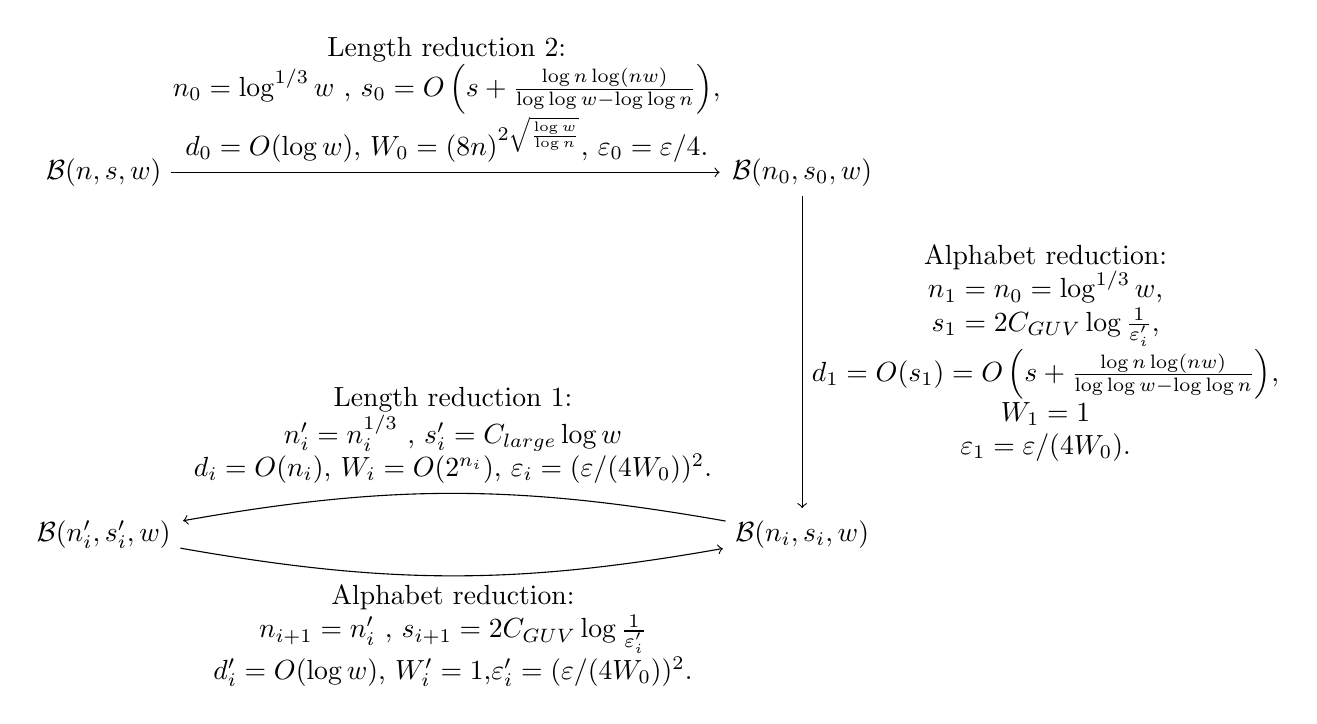
\begin{tikzpicture}[shorten >=1pt, auto]

        \node (q0)   {$\mathcal{B}(n,s,w)$};
        \node[right=7cm of q0] (q1) {$\mathcal{B}(n_0,s_0,w)$};
        \node[below=4cm of q1] (q2) {$\mathcal{B}(n_i,s_i,w)$};
        \node[below=4cm of q0] (q3) {$\mathcal{B}(n'_i,s'_i,w)$};
    
        
        \path[->,align=center]
            (q0) edge node[above] { Length reduction 2:\\
                $n_0 = \log^{1/3}w$ ,  $s_0 = O\left(s+\frac{\log n\log (nw)}{\log\log w-\log\log n}\right)$,\\
                            $d_0 = O(\log w)$,    $W_0 = (8n)^{2\sqrt{\frac{\log w}{\log n}}}$, $\varepsilon_0 = \varepsilon/4$.}(q1);
            (q1);
        \path[->,align=center]
            (q1) edge node[right] {Alphabet reduction:\\
             $n_1 = n_0= \log^{1/3}w$, \\  $s_1 =  2C_{GUV}\log \frac{1}{\varepsilon'_i} $,\\
                            $d_1=O(s_1) =  O\left(s+\frac{\log n\log (nw)}{\log\log w-\log\log n}\right)$,\\    $W_1 = 1$\\ $\varepsilon_1 = \varepsilon/(4W_0)$.                    
                            }(q2);
        \path[->,align=center,bend right=10]
            (q2) edge node[above] {Length reduction 1:\\ $n'_i = n^{1/3}_i$ ,  $s'_i = C_{large} \log w$\\
                            $d_i=O(n_i)$,    $W_i = O(2^{n_i})$, $\varepsilon_i = (\varepsilon/(4W_0))^2$.}(q3);
        \path[->,align=center,bend right=10]
            (q3) edge node[below] {Alphabet reduction:\\ $n_{i+1} = n'_i$ ,  $s_{i+1} = 2C_{GUV}\log \frac{1}{\varepsilon'_i}$\\
                            $d'_{i}=O(\log w)$,    $W'_{i} = 1 $,$\varepsilon'_i = (\varepsilon/(4W_0))^2$.}(q2);
        \end{tikzpicture}
    \caption{The recursion we use to iteratively reduce the ROBP in the construction of the WPRG~\cref{lem:reduction WPRG}.  The arrows represent the reduction from an ROBP to simpler ROBPs. 
    }\label{fig:ROBP reduction}
\end{figure}

The reduction naturally gives a WPRG, which is the PRG in \Cref{lem:reduction WPRG}

\begin{lemma}[Lemma~\ref{lem:reduction WPRG} restated]
    For all $C>0,\varepsilon>1/\poly (w)$, there exists an explicit $\varepsilon$-WPRG for $\mathcal{B}_{(n,C\log w,w)}$ with seed length $O\left(\frac{\log n\log (nw)}{\log\log w-\log\log n}+\log w (\log\log\log w-\log\log\frac{\log w}{\log n/\varepsilon})\right)$ and weight $(8n)^{2\sqrt{\frac{\log w}{\log n}}}$.
\end{lemma}


\begin{proof}
    Let $(\reduct{R},w)$ be the reduction from Lemma~\ref{lem:final reduction}. We construct the WPRG $(G,w)$ with the same weight function $w$ and $G$ is defined as $G(x,i)=\reduct{R}(x,i)$. 
    By \cref{lem:final reduction}, to fool the original ROBP we only need to provide randomness for the seed of $(\reduct{R},w)$ and also provide a random string $x$ which can fool an arbitrary ROBP in  $\mathcal{B}_{(O(1),C_{GUV}\log w,w)}$.
    We use true randomness for $x$ and this only takes $O(\log w)$ random bits.
    Also the randomness used by $(\reduct{R},w)$ is  $O\left(\frac{\log n\log (nw)}{\log\log w-\log\log n}+\log w (\log\log\log w-\log\log\frac{\log w}{\log n/\varepsilon})\right)$.
    So the total seed length is as stated.
    The weight also directly follows from \cref{lem:final reduction}.
\end{proof}

\subsection{Reducing error beyond $1/\poly(w)$} 

To further reduce the error from $1/\poly(w)$ an arbitrary small $\varepsilon$, we use the sampler trick from~\cite{hozaBetterPseudodistributionsDerandomization2021}. The original technique applies to a PRG and gets a WPRG with a smaller error. Here we also use the technique but we apply it on a WPRG and get a WPRG with a smaller error, for the convenience of our analysis.



We shall first introduce the definition of an averaging sampler:

\begin{definition}[Averaging Sampler]\label{def:Sampler}
    A $(\alpha,\gamma)$-averaging sampler is
    a function $\Samp:\{0,1\}^r \times \{0,1\}^p\to \{0,1\}^q$ such that for every function $f:\{0,1\}^q\to [-1,1]$, it holds that:
    \begin{align*}
        \Pr_{x \in \{0,1\}^r }\left[\left|2^{-p}\sum_{y\in \{0,1\}^p}  f(\Samp(x,y)) - \E [f] \right| \ge \alpha\right]\leq \gamma.
    \end{align*}
    
\end{definition}


\begin{lemma}[\cite{chattopadhyayOptimalErrorPseudodistributions2020} Appendix B, \cite{goldreich2011sample, reingold2000entropy}]\label{lem:good sampler}
    For all $\alpha>0,\gamma>0$, there exists an explicit $(\alpha,\gamma)$-averaging sampler with seed length $r=q+O(\log(1/\alpha)+\log(1/\gamma))$ and $p=O(\log(1/\alpha)+\log\log(1/\gamma))$.
\end{lemma}



We now introduce the construction of a WPRG for class $\mathcal{B}_{(n,s,w)}$ with error $\varepsilon$. First, let $(G_0,w_0)$ be a WPRG for $\mathcal{B}_{(n,s,w)}$ with error $1/(2w\cdot (n+1)^2)$ and weight $W$, which is constructed from Lemma~\ref{lem:final reduction}. We then set the parameters as follows:
\begin{itemize}
    \item $k=\frac{\log (n/\varepsilon)}{\log (nw)}$,
    \item $\alpha=1/(W\cdot w^2\cdot (n+1)^2)$,
    \item $\gamma= \varepsilon/(2(2n)^k\cdot (W)^{k+1}\cdot w^2)$.
\end{itemize}
We assume that $\Samp$ is a $(\alpha,\gamma)$-averaging sampler, and let $K,n_{i,j},w_{i,j}$ be as in Lemma~\ref{thm:richardson iteration}.
Our WPRG is constructed as follows:
\begin{align*}
    \begin{cases}
        &G(x,y_1,\ldots,y_{k},i)=G_0(\Samp(x,y_1))_{n_{i,1}}, G_0(\Samp(x,y_2))_{n_{i,2}-n_{i,1}}, \ldots , G_0(\Samp(x,y_{k}))_{n_{i,k}-n_{i,k-1}}\\
        &w(x,y_1,\ldots,y_{k},i)=\sigma_i K\cdot\prod_{j=1}^{k}w_0(\Samp(x,y_j))\\
    \end{cases}
\end{align*}

Now we show that the construction serves as a good WPRG for $\mathcal{B}_{(n,s,w)}$ with error $\varepsilon$. 
\begin{lemma}\label{lem:sampler for small error}
    For all $n,s,w$, assume there exists a $W$-bounded $1/(2w\cdot (n+1)^2)$-WPRG $(G_0,w_0)$  for $\mathcal{B}_{(n,s,w)}$ with seed length $d$, and a $(\alpha,\gamma)$-averaging sampler $\Samp:\{0,1\}^r \times \{0,1\}^p\to \{0,1\}^d$ with $\alpha,\gamma$ as defined above. Then there exists a $\varepsilon$-WPRG for $\mathcal{B}_{(n,s,w)}$ with seed length $r+kp$ and weight $W^{\log(n/\varepsilon)/\log (nw)}\cdot \poly(nw/\varepsilon)$.
\end{lemma}
The proof of \cref{lem:sampler for small error} is deferred to \cref{append:smallererr}.


Combining the lemma with Lemma~\ref{lem:reduction WPRG}, we prove the main theorem of the section:


\begin{theorem}[Theorem~\ref{thm:final WPRG} restated]
    For all integer $n,s,w$, there exists an explicit construction of a $\varepsilon$-WPRG for $\mathcal{B}_{(n,s,w)}$ with seed length 
    $$O\left(s+\frac{\log n\log (nw)}{\log\log w-\log\log n}+\log w (\log\log\log w-\log\log\frac{\log w}{\log n/\varepsilon})+\log(1/\varepsilon)\right)$$ 
    and weight $\poly (nw/\varepsilon)$.
\end{theorem}

\begin{proof}
    Let $(G_0,w_0)$ be a $1/(2w\cdot (n+1)^2)$-WPRG for $\mathcal{B}_{(n,s,w)}$ with seed length 
    $$d=O\left(s+\frac{\log n\log (nw)}{\log\log w-\log\log n}+\log w (\log\log\log w-\log\log\frac{\log w}{\log n/\varepsilon})\right)$$ and weight $W=\poly (nw/\varepsilon)$ given by Lemma~\ref{lem:final reduction}. 
    
    Let $\Samp$ be a $(1/(2W\cdot w^2\cdot (n+1)^2),\varepsilon/(2(2n)^k\cdot W^{k}))$-averaging sampler with seed length $r=d+O(\log(nw/\varepsilon))$ and $p=O(\log(nw)+\log\log(1/\varepsilon))$ given by Lemma~\ref{lem:good sampler}. 

    By Lemma~\ref{lem:sampler for small error}, we get a $\varepsilon$-WPRG for $\mathcal{B}_{(n,s,w)}$ with seed length 
    $$r+(2k+1)p=O\left(s+\frac{\log n\log (nw)}{\log\log w-\log\log n}+\log w (\log\log\log w-\log\log\frac{\log w}{\log n/\varepsilon})+\log(1/\varepsilon)\right)$$ and weight $\poly (nw/\varepsilon)$.


\end{proof}






\section{WPRG for Permutation Read-once Branching Programs}
\label{sec:PROBPWPRG}


In this section we focus on WPRGs against permutation ROBPs. First we recall the definition of permutation ROBPs with only one accept node.
\begin{definition}[Permutation ROBPs]
    A ROBP $f\in \mathcal{B}_{(n,s,w)}$ is a permutation ROBP if for every $i\in [n]$, $x\in \{0,1\}^s$, the matrix $f^{[i-1,i]}(x)$ is a permutation matrix.

    We denote the class of permutation ROBPs with unbounded width and only one accept node by $\mathcal{P}_{(n,s)}$, where $n$ is the length $s$ is the log-size of the alphabet.
\end{definition}
Next we show our WPRG for  $\mathcal{P}_{(n,s)}$.
\begin{theorem}\label{thm:permutation-reduction-main}
    There exists an $\varepsilon$-WPRG for $\mathcal{P}_{(n,s)}$ with seed length $s+O(\log n(\log\log n+\sqrt{\log(1/\varepsilon)})+\log(1/\varepsilon))$ and weight $2^{O(\log n\sqrt{\log(1/\varepsilon)})}$.
\end{theorem}

Before we prove the theorem, we introduce some more definitions and lemmas.
\begin{definition}[PSD norm]
    Let $A$ be a $w\times w$ positive semi-definite matrix. The PSD norm on $\mathbb{R}^w$ with respect to $A$ is defined as $\|x\|_A=\sqrt{x^TAx}$.
\end{definition}


\begin{definition}[sv-approximation \cite{ahmadinejad2023singular}]
    Let $\widetilde{W}$ and $W$ be two $w\times w$ doubly stochastic matrices. We say that $\widetilde{W}$ is a $\varepsilon$-singular-value approximation of $W$, denoted by $\widetilde{W} \sv_{\varepsilon}W$, if for all $x,y\in \mathbb{R}^w$,
    \begin{align*}
        \left|y^T(\widetilde{W}-W)x\right|\leq \frac{\varepsilon}{4}\left( \|x\|^2_{I-W^TW}+\|y\|^2_{I-WW^T}\right).
    \end{align*}
    
\end{definition}

\begin{definition}[fooling with sv-error]\label{def:sv-error}
    Let $(G,w):\{0,1\}^s \rightarrow \{0,1\}^n\times \mathbb{R}$ be a WPRG. Let $\mathcal{C}$ be a family of matrix valued functions $\mathbf{B}: \{0,1\}^s \rightarrow \mathbb{R}^{w\times w}$. We say that $G$ fools $\mathcal{C}$ with $\varepsilon$-sv-error if for all $\mathbf{B}\in \mathcal{C}$, $\sum_{z\in \{0,1\}^s}[\frac{1}{2^s}\mathbf{B}(G(z))\cdot w(x)]\sv_{\varepsilon}\E_{x \in \{0,1\}^n}[\mathbf{B}(x)]$.
\end{definition}


We describe a remarkable previous PRG against permutation ROBPs, given by \cite{hoza2021pseudorandom}. 
From now on we may slightly abuse the notation $\mathcal{P}_{(n,s)}$ to let elements of it also denote matrix-valued functions.
\begin{lemma}[Lemma 4.1 in \cite{chenWeightedPseudorandomGenerators2023}, originally by  \cite{hoza2021pseudorandom}]\label{lem:sv-fool}
    For all $s,n,\varepsilon$ there exists a PRG (actually the INW generator) that fools $\mathcal{P}_{(n,s)}$ with $\varepsilon$-sv-error. The seed length is
    \begin{align*}
        s+O(\log n(\log\log n+\log(1/\varepsilon))).
    \end{align*} 
\end{lemma}
\begin{remark}
    We note that Lemma 4.1 in \cite{chenWeightedPseudorandomGenerators2023} only proves the case for $s=2$, but their proof can naturally be generalized to handle arbitrary $s$.  See \cref{sec:sv-fool sketch}.
\end{remark}

Next we describe the key ingredient in previous error reductions for WPRGs against permutation ROBPs. 

\begin{lemma}[Claim 9.3 in \cite{chenWeightedPseudorandomGenerators2023}]\label{lem:sv-error-reduction-polynomials}
    Let $n \in \mathbb{N}$, let $\tau \in \left(0, \frac{1}{64 \log^2 n}\right)$, and let $G:\{0,1\}^d\to (\{0,1\}^s)^n$ be a PRG that fools  $\mathcal{P}_{(n,s)}$ with sv-error $\tau$. Let $k \in \mathbb{N}$, and let 
    \[
    \alpha = \left(4 \cdot \sqrt{\tau} \cdot \log n \right)^{k+1}.
    \]
    Then there exists a WPRG $G^{(k)}, w^{(k)}$ that can be written in the form of 
    \begin{align*}
        &G^{(k)}(i, x_1, \ldots, x_r)=G(x_1)_{n_{i,1}}, G(x_2)_{n_{i,2}}, \ldots,G(x_r)_{n_{i,r}}, \\
        &w^{(k)}(i)=\sigma(i)\cdot K.
    \end{align*}
    where $K=n^{O(k)},i\in [K],r=O(k\log n)$, $\sigma(i)\in \{-1,0,1\}$ and $0\leq n_{i,j}\leq n$, such that $G^{(k)}$ fools $\mathcal{P}_{(n,s)}$ with entrywise error $\alpha$.

    
\end{lemma}






\subsection{One level of the reduction}
  We show that the previous lemma already gives a reduction:
\begin{lemma}\label{lem:onelevelWPRPerm}
    For any integer $n,k,s$ and any $\varepsilon>0$, there exists $\tau=\Omega(\varepsilon^{\frac{2}{k+1}}/\log^2 n)$ such that there exists a $(O(k\log n), n^{O(k)},\varepsilon)$-weighted pseudorandom reduction $(\reduct{R},w)$ from $\mathcal{P}_{(n,s)}$ to $\mathcal{P}_{(O(k\log n),s+O(\log n(\log\log n+\log 1/\tau)))}$.
\end{lemma}



\begin{proof}
    Let $G$ be the INW PRG that fools $\mathcal{P}_{(n,s)}$ with $\tau$-sv-error, such that $\tau=\min\{\frac{\varepsilon^{2/(k+1)}}{16\log^2 n},\frac{1}{64\log^2 n}\}$. Then the seed length is $d = s+O(\log n(\log\log n+\log 1/\tau))$ by Lemma \ref{lem:sv-fool}.

    We invoke \cref{lem:sv-error-reduction-polynomials} with $G$ and $k$, which gives $(G^{(k)},w^{(k)})$. This WPRG fools $\mathcal{P}_{(n,s)}$ with entrywise error $\left(4 \cdot \sqrt{\tau} \cdot \log n \right)^{k+1}<\varepsilon$. We define the reduction $(\reduct{R},w): \reduct{R}_i(x_1,...,x_r)=G^{(k)}(i,x_1,...,x_r),w_i=w^{(k)}(i)$.

    By \cref{lem:sv-error-reduction-polynomials}, the weight of this reduction is bounded by $K=n^{O(k)}$. 
    The seed length of the reduction is $\log K=O(k\log n)$, since we need $\log K=O(k\log n)$ bits to choose $i$.

    Given any $f\in \mathcal{P}_{(n,s)}$, notice that each $f\circ \reduct{R}_i$ is a ROBP of length $r=O(k\log n)$ and alphabet size $2^d=2^{s+O(\log n(\log\log n+\log 1/\tau))}$. The reason is that the transition matrix of $f\circ \reduct{R}_i$ from the $j-1$-th layer to the $j$-th layer on input $x\in \{0,1\}^{d}$ can be expressed as $(f\circ \reduct{R}_i)^{[j-1,j]}(x)$. As $(f\circ \reduct{R})^{[j-1,j]}(x)=f^{[n_{i,j-1},n_{i,j}]}(G(x)_{n_{i,j}-n_{i,j-1}})$ and the latter is a product of $n_{i,j}-n_{i,j-1}$ permutation matrices, the transition matrix of $f\circ \reduct{R}_i$ is also a permutation matrix. Hence $f\circ \reduct{R}_i$ is a permutation ROBP.
    Also, note that each $f\circ \reduct{R}_i$ only has one accept node since its accept node is the same as that of $ f$.
    
    Therefore, the reduction is a $(O(k\log n), O(n^k),\varepsilon)$-weighted pseudorandom reduction.
    
\end{proof}


Setting $k=\sqrt {\log (1/\varepsilon)}$ in \cref{lem:onelevelWPRPerm}, we immediately have the following lemma:
\begin{lemma}\label{cor:permutation-reduction-1}
    For any integer $n,s$ and any $\varepsilon>0$, there exists a $(O(\log n\sqrt{\log (1/\varepsilon)}),2^{O(\log n\sqrt{\log (1/\varepsilon)})},\varepsilon)$-weighted pseudorandom reduction from $\mathcal{P}_{(n,s)}$ to $\mathcal{P}_{(O(\log n\sqrt{\log (1/\varepsilon)}),s+O(\log n(\sqrt{\log (1/\varepsilon)}+\log \log n)))}$.
\end{lemma}

Setting $k=O(\log^2 n)$ in \cref{lem:onelevelWPRPerm}, we immediately have the following lemma:
\begin{lemma}\label{cor:permutation-reduction-2}
    For any integer $n,s$ and $\varepsilon>0$, there exists a $(O(\log^3 n),2^{O(\log^3 n)},\varepsilon)$-weighted pseudorandom reduction from $\mathcal{P}_{(n,s)}$ to  $\mathcal{P}_{(\log^3 n,s+O(\frac{\log (1/\varepsilon)}{\log n}+\log n\log \log n))}$.
\end{lemma}




\subsection{Recursion of reductions}
We give a multi-level recursive procedure which gradually reduces the program from $\mathcal{P}_{(n,s)}$ to $\mathcal{P}_{(O(1),s+O(\log n(\log\log n+\sqrt{\log(1/\varepsilon)})))}$ with error $\varepsilon$, for any $n,s,\varepsilon$. 

We start by reducing the length of the permutation ROBP to $O(\log n\sqrt{\log(1/\varepsilon)})$ and the weight to $2^{O(\log n\sqrt{\log(1/\varepsilon)})}$ with error $\varepsilon/2$. Previous works use an INW PRG to fool the reduced ROBP, which leads to an extra double logarithmic factor in the seed length. Here we use the recursion instead to avoid this extra factor. 



\begin{lemma}[Reduction for permutation ROBP]\label{lem:permutation-reduction-main}
    For any integer $n,s$ and any $\varepsilon>0$, there exists a $\left( O(\log n\sqrt{\log(1/\varepsilon)}),2^{\log n\sqrt{\log(1/\varepsilon)}},O(\varepsilon) \right)$-weighted pseudorandom reduction from $\mathcal{P}_{(n,s)}$ to $\mathcal{P}_{(O(1),s+O(\log n(\log\log n+\sqrt{\log(1/\varepsilon)})+\log(1/\varepsilon)))}$.
\end{lemma}




\begin{proof}

    Let $(\reduct{R}^{(0)},w^{(0)}$ be the $(d_0,W_0,\varepsilon/2)$-weighted pseudorandom reduction from $\mathcal{P}_{(n,s)}$ to $\mathcal{P}_{(n_1,s_1)}$  such that $n_1=O(\log n\sqrt{\log(1/\varepsilon)})$ and $s_1=s+O(\log n(\log\log n+\sqrt{\log(1/\varepsilon)}))$. The reduction is guaranteed by Lemma \ref{cor:permutation-reduction-1} and have the following parameters: 
    \begin{enumerate}
        \item $d_0=O(\log n\sqrt{\log(1/\varepsilon)})$,
        \item $W_0=2^{O(\log n\sqrt{\log(1/\varepsilon)})}$.
    \end{enumerate}

    Now we define a new parameter $\varepsilon'=\varepsilon/2W_0$. Let 
    \[n_0=n,n_i=\log^3 n_{i-1}\]
    for each $i=1,\ldots,l$ and $n_l= 32768$. It is clear that $l\leq \log\log n$.

    For each $i=1,\ldots,l$, let $(\reduct{R}^{(i)},w^{(i)})$ be the $(d_i,W_i,(\varepsilon')^2)$-weighted pseudorandom reduction from $\mathcal{P}_{(n_{i},s_{i})}$ to $\mathcal{P}_{(n_{i+1},s_{i+1})}$, which is guaranteed by Lemma \ref{cor:permutation-reduction-2}. The reduction has the following parameters:
 
    \begin{enumerate}
        \item $d_i=O(\log^3 n_{i})$,
        \item $W_i=2^{\log^3 n_i}$,
        \item $s_{i+1}=s_{i}+O(\frac{\log(1/\varepsilon')}{\log n_{i}}+\log n_{i}\log \log n_{i})=s_{i}+O(\frac{\log(1/\varepsilon)}{\log n_{i}})$.
    \end{enumerate}

    Using \cref{lem:multi composition}, we first composite $(\reduct{R}^{(1)},w^{(1)}),\ldots,(\reduct{R}^{(l)},w^{(l)})$ to get a $(d^*,W^*,\varepsilon^*)$-weighted pseudorandom reduction $(\reduct{R}^{(*)},w^{(*)})$ from $\mathcal{P}_{(n_0,s_0)}$ to $\mathcal{P}_{(n_l,s_l)}$ with $\reduct{R}^{(*)}=\reduct{R}^{(1)}\circ \ldots \circ \reduct{R}^{(l)}$ and $w^{(*)}=w^{(1)}\cdot \ldots \cdot w^{(l)}$. We have the following parameters:

    \begin{enumerate}
        \item $d^*=d_1+\ldots+d_l\leq O(l\log^3 n_1)\leq O(\log^{0.1}(n/\varepsilon))$,
        \item $W^*=W_1\cdot \ldots \cdot W_l\leq 2^{O(l\cdot \log^3n_1)}\leq 2^{O(\log^{0.1}(n/\varepsilon))}$,
        \item $\varepsilon^*=\sum_{i=1}^{l}(\varepsilon')^{2}\cdot \prod_{j=0}^{i-1}W_j\leq(\varepsilon')^{2}\cdot W^*\cdot l\leq \varepsilon'/2$,
        \item $s_l=s_0+\sum_{i=1}^{l}(s_i-s_{i-1})=s_0+\sum_{i=1}^{l}O(\frac{\log(1/\varepsilon')}{\log n_{i}})=s_0+O(\log 1/\varepsilon')$.
    \end{enumerate}

    The last item holds because $n_i$ decreases rapidly. Because $n_{i-1}= 2^{\sqrt[3]{n_i}}$, when $n_i\geq 2^{15}=32768$, We have $n_{i-1}\geq n^2_i$. When $n_l\geq 32768$, $\sum_{i=1}^{l}\frac{\log(1/\varepsilon')}{\log n_{i}}\leq \log 1/\varepsilon'\cdot (1/\log n_l+1/(2\log n_l)+1/(4\log n_l)+\cdots +1/(2^l\log n_l))\leq \log 1/\varepsilon'$. 

    Finally, we composite $(\reduct{R}^{(*)},w^{(*)})$ with $(\reduct{R}^{(0)},w^{(0)})$ to get the final reduction $(\reduct{R},w)$ from $\mathcal{P}_{(n,s)}$ to $\mathcal{P}_{(O(1),s_l))}$. 
    By \cref{lem:composition}, the parameters are:
    \begin{enumerate}
        \item $d=d^*+d_0=O(\log n\sqrt{\log(1/\varepsilon)})$,
        \item $W=W^*\cdot W_0\leq 2^{O(\log n\sqrt{\log(1/\varepsilon)})}$,
        \item $\varepsilon=\varepsilon/2+\varepsilon'/2\cdot W_0\leq \varepsilon$,
        \item $s=s_l=s_0+O(\log 1/\varepsilon')=s+O(\log n(\log\log n+\sqrt{\log(1/\varepsilon)})+\log(1/\varepsilon))$.
    \end{enumerate}
\end{proof}
One can also see our reduction strategy for the above lemma through Figure \ref{fig:WPRGforPerm}.
\begin{figure}[H]\label{fig:WPRGforPerm}
    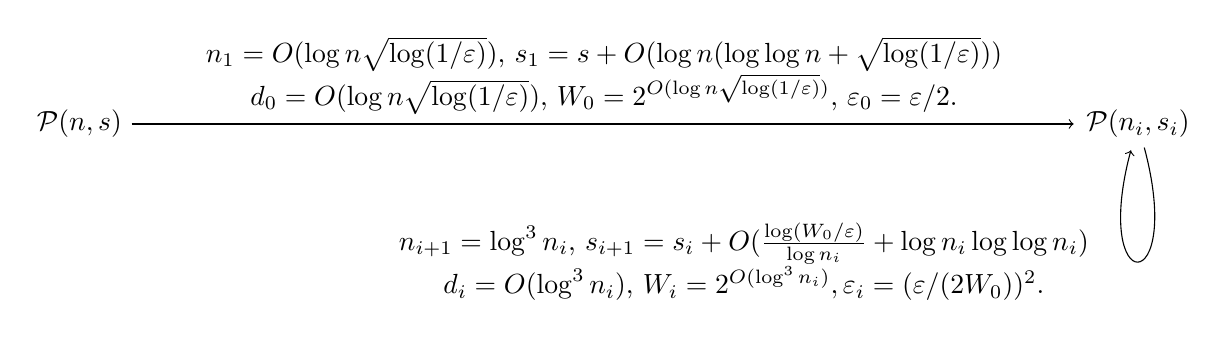
\begin{tikzpicture}[shorten >=1pt, auto]

    \node (q0)   {$\mathcal{P}(n,s)$};
    \node[right=12cm of q0] (q1) {$\mathcal{P}(n_i,s_i)$};

    

    \path[->,align=center]
        (q0) edge node[above] {
            $n_1=O(\log n \sqrt{\log(1/\varepsilon)})$, $s_1 = s+O(\log n (\log\log n+\sqrt{\log(1/\varepsilon)}))$\\
                        $d_0 = O(\log n \sqrt{\log(1/\varepsilon)})$,    $W_0 = 2^{O(\log n \sqrt{\log(1/\varepsilon)})}$, $\varepsilon_0 = \varepsilon/2$.}(q1);
        (q1);
    \path[->,loop below,align=center, distance=2cm]
        (q1) edge node[left=0.5cm] 
         {
            $n_{i+1}=\log^3 n_i$, $s_{i+1} = s_i+O(\frac{\log(W_0/\varepsilon)}{\log n_i}+\log n_i\log\log n_i)$\\
                        $d_i = O(\log^3 n_i)$,    $W_i = 2^{O(\log^3 n_i)}, \varepsilon_i = (\varepsilon/(2W_0))^2$.                    
                        }(q1);

    \end{tikzpicture}
    \caption{Reduction for permutation ROBPs in~\cref{lem:permutation-reduction-main}. 
    }
\end{figure}


Given this lemma, we immediately have the main theorem of this section:

\begin{theorem}[Theorem \ref{thm:permutation-reduction-main} restated]
    There exists an $\varepsilon$-WPRG for $\mathcal{P}_{(n, s)}$ with seed length $s+O(\log n(\log\log n+\sqrt{\log(1/\varepsilon)})+\log(1/\varepsilon))$ and weight $2^{O(\log n\sqrt{\log(1/\varepsilon)})}$.
\end{theorem}

\begin{proof}
    Let $(\reduct{R}, w)$ be the reduction from Lemma \ref{lem:permutation-reduction-main}. We construct the WPRG $(G,w) $ with the same weight function $w$, and $G$ is defined as $G(x,i)=\reduct{R}(x,i)$.
    By \cref{lem:permutation-reduction-main},  to fool the original ROBP we only need to provide randomness for the seed of $(\reduct{R},w)$ and also provide a random string $x$ which can fool an arbitrary ROBP in  $\mathcal{P}_{(O(1),s+O(\log n(\log\log n+\sqrt{\log(1/\varepsilon)})+\log(1/\varepsilon)))}$.
    We can use another $\varepsilon$ error INW generator from \cite{hozaPseudorandomGeneratorsUnboundedWidth2020} to generate this constant length $x$ and this only takes $s + O\left(\log n(\log\log n+\sqrt{\log(1/\varepsilon)})+\log(1/\varepsilon) \right)$ random bits.
    Also the randomness used by $(\reduct{R},w)$ is $O(\log n\sqrt{\log(1/\varepsilon)})$.
     So the total seed length is as stated.
     The weight also directly follows from \cref{lem:permutation-reduction-main}.



\end{proof}





It is well known that a WPRG fools a Permutation ROBP with an arbitrary number of accept nodes and error $\varepsilon$ if it fools the program with only one accept node with error $\varepsilon/w$. Therefore, we have the following corollary:

\begin{theorem}
    There exists an $\varepsilon$-WPRG for length $n$, width $w$, alphabet size (out degree) $2^s$ Permutation ROBPs having an arbitrary number of accept nodes, with seed length $s+O(\log n(\log\log n+\sqrt{\log(w/\varepsilon)})+\log(w/\varepsilon))$ and weight $2^{O(\log n\sqrt{\log(w/\varepsilon)})}$.
\end{theorem}







\section{Derandomizing Regular Branching Programs}\label{sec:derand regular}



In this section, we give our improved derandomization for short-wide regular ROBPs.
When $n\leq 2^{\log^{1/2} w}$ and $\varepsilon=1/\poly(w)$, our result provides an $O(\log \frac{w}{\eps})$ space derandomization, which is optimal up to a constant factor. 
We achieve this by constructing a new derandomization algorithm that runs in space $O(\log(w/\varepsilon)+\log n\sqrt{\log (w/\epsilon)})$, adapted from our WPRG for permutation ROBPs from the \cref{sec:PROBPWPRG}.

We remark that for the special case of binary regular ROBPs, one can transform them to permutation ROBPs in logspace, see \cref{sec:binaryRegulartoPerm}, and then run the WPRG of the previous section.
But for the general case, i.e. arbitrary alphabet size, the problem turns out to be more complex. 
In the rest of this section, we mainly focus on the general case.



\subsection{More preliminaries}

We recall some standard definitions in the literature of  \cite{reingold2000entropy, rozenmanDerandomizedSquaringGraphs2005, ahmadinejadHighprecisionEstimationRandom2022, chenWeightedPseudorandomGenerators2023, chattopadhyayRecursiveErrorReduction2023}. 


\begin{definition}[Regular bigraph]
    A bigraph is a triple $G=(U,V,E)$, where $U$ and $V$ are two sets of vertices and $E\subseteq U\times V$ is a set of edges going from $U$ to $V$. A bigraph is called $d$-regular if every vertex in $U$ has $d$ outgoing edges and every vertex in $V$ has $d$ incoming edges. 

    The transition matrix of a regular bigraph is a the matrix $\mathbf{M}\in \mathbb{R}^{V\times U}$ such that $\mathbf{M}_{v,u}$ is the fraction of edges going from $u$ that go to $v$.

\end{definition}

\begin{definition}[One-way labeling]
    A one-way labeling of a $d$-regular bigraph $G$ assigns a label $i\in [d]$ to each edge in $G$ such that for every vertex $u\in U$, the labels of the outgoing edges of $u$ are distinct. If $G$ has a one way labeling, we say that $G[u,i]=v$ if the outgoing edge of $u$ that is labeled $i$ goes to $v$.
\end{definition}

\begin{definition}[Two-way labeling]
    A two-way labeling of a $d$-regular bigraph $G$ is a labeling of the edges of $G$ such that:
    \begin{itemize}
        \item Every edge $(u,v)$ has two labels in $[d]$, the `outgoing label' and the `incoming label'.
        \item For every vertex $u\in U$, the outgoing labels of the outgoing edges of $u$ are distinct.
        \item For every vertex $v\in V$, the incoming labels of the incoming edges of $v$ are distinct.
    \end{itemize}
\end{definition}



\begin{definition}[Rotation map]\label{def:rot map}
    Let $G=(U,V,E)$ be a $d$-regular bigraph with a two-way labeling. The rotation map of $G$ is a function $\Rot_G:U\times [d]\to  V\times [d]$ such that $\Rot_G(u,i)=(v,j)$ if there is an edge $(u,v)\in E$ with the outgoing label $i$ and the incoming label $j$.
    
\end{definition}


\begin{definition}[Derandomized Product]
    Let $G_1=(U,V,E_1)$ and $G_2=(V,T,E_2)$ be two $d$-regular bigraphs where $G_1$ has a two-way labeling and $G_2$ has a one-way labeling. Let $H=([d],[d],E_H)$ be a $c$-regular bigraph with one way labeling. The derandomized product of $G_1$, $G_2$ and $H$ is a $(c\cdot d)$-regular bigraph with one-way labeling denoted by $G_1\ds_H G_2$ defined as follows. To compute $(G_1\ds_H G_2)[v_0,(i_0,j_0)]$ for  $v_0\in U$ and $(i_0,j_0)\in [d]\times [c]$:
    \begin{itemize}
        \item Let $(v_1,i_1)=\Rot_{G_1}(v_0,i_0)$.
        \item Let $i_2=H[i_1,j_0]$.
        \item Let $v_2=G_2[v_1,i_2]$.
        \item Output $(G_1\ds_H G_2)[v_0,(i_0,j_0)]=:v_2$.
    \end{itemize}
    
\end{definition}


\begin{definition}[Two-way labeling of derandomized product]
    Let $G_1=(U,V,E_1)$ and $G_2=(V,T,E_2)$ be two $d$-regular bigraphs where both $G_1$ and $G_2$ have two-way labeling. Let $H=([d],[d],E_H)$ be a $c$-regular bigraph with two-way labeling. We define the two-way labeling of the derandomized product $G_1\ds_H G_2$ as follows. To compute the rotation map $\Rot_{G_1\ds_H G_2}$ for any vertex $v_0\in U$ and any pair $(i_0,j_0)\in [d]\times [c]$, we do the following:
    \begin{itemize}
        \item Let $(v_1,i_1)=\Rot_{G_1}(v_0,i_0)$.
        \item Let $(i_2,j_1)=\Rot_H(i_1,j_0)$.
        \item Let $(v_2,i_3)=\Rot_{G_2}(v_1,i_2)$.
        \item Output $\Rot_{G_1\ds_H G_2}(v_0,(i_0,j_0))=(v_2,(i_3,j_1))$.
    \end{itemize}
    
\end{definition}

To ensure that the derandomized product behaves like the direct concatenation of the two bigraphs, we need $H$ to be a spectral expander. 

\begin{definition}[spectral expander]
    Let $H=(U,V,E_H)$ be a $d$-regular bigraph with transition matrix $W_H\in \mathbb{R}^{U\times V}$, where $|U|=|V|$. Define $J\in \mathbb{R}^{U\times V}$ where $J_{i,j}=1/|U|$ for all $i\in U,j\in V$. Then the spectral expansion of $H$ is denoted by $\lambda(H)$ and defined as follows:
    \begin{align*}
        \lambda(H)=\|W_H-J\|_2
    \end{align*}
\end{definition}



We also need the definitions for regular branching programs:

\begin{definition}[Regular Branching Program]
    Let $f$ be a ROBP in $\mathcal{B}_{n,s,w}$. We call $f$ a regular branching program if all vertices in the graph of $f$ except the vertices in the first layer have precises $2^s$ incoming edges.
\end{definition}

A general regular branching program may not have a two-way labeling. If we equip it with a two-way labeling for each step of the transition, we call it a regular ROBP with two-way labeling.

\begin{definition}[Regular ROBP with Two-way labeling]\label{def:regular label}
    A regular ROBP with two-way labeling is a pair $(f,\ell_{in})$ where $f$ is a regular ROBP in $\mathcal{B}_{n,s,w}$ with  vertex set $V=V_0\cup V_1\cup \cdots \cup V_n$,  edge set $E=E_1\cup\cdots \cup E_n$ and edge labeling $\ell_{out}:E\to [2^s]$. The function $\ell_{in}:E\to [2^s]$ map every edge to another label. Furthermore, for every vertex $i \in [n]$, $l_{in}$ and $l_{out}$ restricted on $E_i$ is a two-way labeling of the bigraph $G_i:=(V_{i-1},V_i,E_i)$.
    
    We neglect $\ell_{out}$ in the notation since we can always consider $\ell_{out}$ to be the canonical order given by the ROBP.

    We denote the class of all regular ROBPs with two-way labeling $\mathcal{R}^{tw}_{n,s,w}$.
\end{definition}



We recall the derandomization algorithm for regular branching programs in \cite{chenWeightedPseudorandomGenerators2023}.

Let $(f,\ell_{in})$ be a regular ROBP with two-way labeling in $\mathcal{R}^{tw}_{n,s,w}$. For each $i\in [\log n]$, let $H_t=([2^s\cdot c^{t-1}],[2^s\cdot c^t],E_{H_t})$ be a $c$-regular bigraph with $\lambda(H_t)\leq \lambda$. Define $\widetilde{G}_{j\to j+1}:=(V_{t-1},V_t,E_t)$, which is a $2^s$-regular bigraph with two-way labeling. Define $E(SC_n)=\{(j,j+2^t):j\in [n-2^t],t\in [\log n], 2^t \text{ is the largest power of 2 dividing } j\}$. For each $(j,j+2^t)\in E(SC_n)$ recursively define the graph $\widetilde{G}_{j \to j+2^t}$ as follows:
\begin{align*}
    \widetilde{G}_{j\to j+2^t} := \widetilde{G}_{j\to j+2^{t-1}}\ds_{H_i} \widetilde{G}_{j+2^{t-1}\to j+2^t}
\end{align*}



The following lemma shows that the transition matrix of the final graph $\widetilde{G}_{0\to n}$ is close to the product of the transition matrices of the intermediate graphs.

\begin{lemma}[Lemma A.20 of \cite{chenWeightedPseudorandomGenerators2023}] \label{lem:sv approximation algorithm}
    Let $n, d, c \in \mathbb{N}$. For each $t \in \{0, 1, \ldots, \log n\}$ and each $j \in [n-2^t]$, let $\widetilde{G}_{j+2^{t-j}} = \big(V_j, V_{j+2^t}, E_{j+2^{t-j}}\big)$ be a $(d \cdot c^t)$-regular bigraph with a two-way labeling. Furthermore, let $\lambda \in \big(0, \frac{1}{6 \log^2 n}\big)$, and for each $t \in [\log n]$, let $H_t = \big([d \cdot c^{t-1}], [d \cdot c^{t-1}], E_{H_t}\big)$ be a $c$-regular bigraph with a one-way labeling satisfying $\lambda(H_t) \leq \lambda$. Assume also that for each $t \in [\log n]$ and each $j \in [n-2^t]$, we have
\[
\widetilde{G}_{ j \to j+2^t} = \widetilde{G}_{ j \to j+2^{t-1}} \ds_{H_t} \widetilde{G}_{j+2^{t-1}\to j+2^t}, \forall t \ge 1,
\]
and 
\[
\widetilde{G}_{ j \to j+1} = G_{j \to j+1},
\]
(where the equation above merely denotes equality as graphs with one-way labelings). For each $(i, j) \in E(\mathsf{SC}_n)$, let $\widetilde{\mathbf{W}}_{j\gets i}$ be the transition matrix of $\widetilde{G}_{i\to j}$, and let 
\[
\mathbf{W}_{j\gets i} = \widetilde{\mathbf{W}}_{j\gets j-1} \cdots \widetilde{\mathbf{W}}_{i+1\gets i}
\] 
Then 
\[
\widetilde{\mathbf{W}}_{n\gets 0} \sv_{11\lambda \cdot \log n} \mathbf{W}_{n\gets 0}.
\]
    
\end{lemma}


\begin{theorem}[Claim A.23 of \cite{chenWeightedPseudorandomGenerators2023}] \label{thm:derandomization algorithm}
    The following algorithm computes 
    $$\Rot_{\widetilde{G}_{0\to n}}(v_0, (x,e_1, \ldots, e_{\log n}))$$

\begin{enumerate}
    \item For $i = 1$ to $n$:
    \begin{enumerate}
        \item[(a)] Update $(v, x) \gets \Rot_{\widetilde{G}_{i-1\to i}}(v, x)$, so now $v \in V^{(i)}$.
        \item[(b)] If $i < n$:
        \begin{enumerate}
            \item Let $t \in [\log n]$ be the smallest positive integer such that $i$ is not a multiple of $2^t$, i.e., the binary expansion of $i$ has precisely $t-1$ trailing zeroes.
                
            \item Update $(x,e_1, \ldots, e_{t-1}) \gets \Rot_{H_t}((x,e_1, \ldots, e_{t-1}), e_t)$.
        \end{enumerate}
    \end{enumerate}
    \item Output $(v, e)$.
\end{enumerate}






\end{theorem}


We also need the efficiently computable spectral expander $H_t$. The following lemma shows that such a spectral expander exists. The construction of $H_t$ is based on Margulis-Gabber-Galil graphs \cite{margulis1973explicit, gabber1981explicit}.

\begin{lemma}[Space-efficient expanders, Lemma A.22 of \cite{chenWeightedPseudorandomGenerators2023}] \label{lem:space-efficient expanders}
\label{lem:HExpander}
    For every $d \in \mathbb{N}$ that is a power of two, for every $\lambda \in (0, 1)$, there is a bigraph $H = \big([d], [d], E_H\big)$ with a two-way labeling satisfying the following:
    \begin{itemize}
        \item $\lambda(H) \leq \lambda$.
        \item $H$ is $c$-regular where $c$ is a power of two and $c \leq \mathrm{poly}(1 / \lambda)$.
        \item $\mathrm{Rot}_H$ can be evaluated in space that is linear in its input length, i.e., space $O(\log(d / \lambda))$.
    \end{itemize}
\end{lemma}


We use the following error reduction polynomial in our algorithm, which gives a good sv-approximation for a sequence of transitions.


\begin{theorem}[Recursion  \cite{chattopadhyayRecursiveErrorReduction2023}]\label{lem:derandErrorRedPoly} 
    Let $\{A_i\}_{i=1}^n\subset \mathbb{R}^{w\times w}$ be a sequence of doubly stochastic matrices. Let $\{B_{i,j}\}_{i,j=0}^n \subset \mathbb{R}^{w\times w}$ be a family of matrices such that $B_{i,j} \sv_{\varepsilon/(10\log n)} A_{i+1}\ldots A_j$ Assuming that $B_{i-1,i}=A_i$ for all $i$.  Then for any $k\in \mathbb{N}$, there exists $K=O((2n)^k)$, $t=O(k\log n)$, a set of indices $n_{i,j}$ for each $i\in [K],j\in [t]$ with $0\leq n_{i,1}\leq \ldots\leq n_{i,t}= n$ and a set of signs $\sigma_i\in\{-1,0,1\}$ for each $i\in [K]$ such that:
    \begin{align*}
        \sum_{i\in [K]}\sigma_i\cdot B_{0,n_{i,1}}B_{n_{i,1},n_{i,2}}\ldots B_{n_{i,t-1},n_{i,t}}\sv_{\varepsilon^k } A_1A_2\ldots A_n.
    \end{align*}

\end{theorem}







\subsection{The algorithm}


We give our derandomization algorithm for regular branching programs. 

\begin{theorem}
    There exists an algorithm that takes as input a regular ROBP and a parameter $\varepsilon>0$, and outputs an approximation of its acceptance probability with error $\varepsilon$. Furthermore, if the regular ROBP has length $n$, width $w$ and alphabet size $2^s$, then the algorithm runs in space $O(s+\log n(\log\log n+\sqrt{\log(w/\varepsilon)})+\log(w/\varepsilon))$.
\end{theorem}

\begin{proof}
    To define the algorithm, we need to prepare three things in advance: the two-way labeling, the error reduction, and the rotation algorithm.

    First, the input of the algorithm is a regular ROBP $f$ without two-way labeling. However, we can easily convert it to a regular ROBP $G$ with two-way labeling by assigning an arbitrary label to each incoming edge. (i.e., $\ell_{in}(e)=i$ if $e$ is the $i$-th incoming edge of the vertex.). This can be done in space $O(s+\log(nw))$.
    

    Second, we need to predetermine the sets of indices and signs used in a recursive error reduction procedure. We use parameters similar to those in \cref{sec:PROBPWPRG}. 
    We set $n_0=n,n_1=O(\log n\sqrt{\log (w/\varepsilon)})$. 
    For $i=2,3,\ldots$, let $n_i=\left\lceil \log^3 n_{i-1}\right\rceil$. We take $l$ to be the first integer such that $n_l\le 2^{15}$. 
    Notice that $l=o(\log\log n)$.
  
    Now for each $i\in [l]$, we prepare a group of parameters for invoking \cref{lem:derandErrorRedPoly}. We use $n_{i},n_{i+1}$ as the $n,r$ respectively in \cref{lem:derandErrorRedPoly}. When we apply it to $n_0,n_1$, we set $\alpha_0=\varepsilon/2w$ as the target error and $k_0=\sqrt{\log(1/\alpha_0)}$, $\tau_0=\min\{\frac{\varepsilon^{2/(k_0+1)}}{16\log^2 n_0},\frac{1}{64\log^2 n_0}\}$ as the original error. 
    \cref{lem:derandErrorRedPoly} gives a number $W_0\in \mathbb{N}$,a set of indices $\{n^{(0)}_{j,t}\}_{j\in [W_0],t\in [n_1]}$ and a set of signs $\{\sigma_{j}\}_{j\in [W_0]}$.
    After that, we set $\varepsilon'=\varepsilon^2/(2wW_0)$.
    Then for every $i\in [l-1]$, we set $\alpha_i=\varepsilon'$  and $k_i=\log^2 n_i$, $\tau_i=\min\{\frac{(\varepsilon')^{2/(k_i+1)}}{16\log^2 n_{i}},\frac{1}{64\log^2 n_{i}}\}$. \cref{lem:derandErrorRedPoly} gives a number $W_i\in \mathbb{N}$, a set of indices $\{n^{(i)}_{j,t}\}_{j\in [W_i],t\in [n_{i+1}]}$ and a set of signs $\{\sigma_{j}\}_{j\in [W_i]}$.

    We stress that one can assume each $\{n^{(i)}_{j,t}\}_{j\in [W_i],t\in [n_{i+1}]}$ and $\{\sigma_{j}\}_{j\in [W_i]}$ satisfies the following properties:

    For each $i = 0, 1, 2, \ldots, l-1$, for any doubly stochastic matrices $A_1,\ldots,A_{n_i}$ and $B_{j,q}$ such that $B_{p,q}\sv_{\tau_i}A_{p+1}\ldots A_q$ and $B_{p-1,p}=A_p$ for all $p\in [n_i]$.
    Then let 
    \[
        A'=\sum_{j\in [W_i]}\sigma_j\cdot B_{0,n^{(i)}_{j,1}}B_{n^{(i)}_{j,1},n^{(i)}_{j,2}}\ldots B_{n^{(i)}_{j,n_{i+1}-1},n^{(i)}_{j,n_{i+1}}}.
    \]
    It holds that $A'$ approximates $A_1\ldots A_{n_i}$ with entry-wise error at most $\alpha_i$, by \cref{lem:derandErrorRedPoly}.


    The third part of the preparation is an implementation of the rotation algorithm \cref{thm:derandomization algorithm}. 
    We use the algorithm for every level $i$, to get those approximation matrices with sv-error $\tau_i$.
  
    
    For any $i= 0, 1, 2,\ldots, l-1$, to use \cref{lem:sv approximation algorithm} for the correctness of \cref{thm:derandomization algorithm}, we need to prepare a group of parameters $n_i, \lambda_i, d_i, c_i$. 
    Let $\lambda_i$ be $\tau_i/(11\log n_i)$. 
    For each $t\in [\log n_i]$, we use $H^{(i)}_t$ as the $t$-th $\lambda_i$-spectral expander used in the lemma, where every $H^{(i)}_t$ can be achieved by \cref{lem:HExpander}. 
    The parameter $c_i$ is set to be the degree of $H^{(i)}_t$, which is the same for all $t$.
    We let $d_0 = 2^s$.
    Let $d_{i+1}=d_{i}+\left\lceil \log n_i\right\rceil \cdot \left\lceil \log c_i\right\rceil$ for all $i = 0, 1, \ldots, l-1$.
    One can see later that the parameter $d_i$ is the degree of the branching program after the first $i$ levels of reduction.

    Now we have prepared $l,\{n_i\}_{i=0}^l,\{W_i\}_{i=0}^l,\{n^{(i)}_{j,t}\}_{i\in [l],j\in [W_i],t\in [n_{i+1}]},\{\sigma_{j}\}_{j\in [n_i]},\{d_i\}_{i=0}^l,\{c_i\}_{i=1}^l$ and graphs  $\{H^{(i)}_t\}_{i\in [l],t\in [\log n_i]}$. 
    Notice that all these parameters can be computed in logspace, so we will directly use them in the algorithm description.
    Then we construct our algorithm  that approximates the acceptance probability of the regular ROBP.
    In general the algorithm adapts the WPRG of the previous section and runs the ROBP on the output of the WPRG but with the following two adjustments:
    \begin{itemize}
        \item every time when the WPRG needs to conduct a one-step walk on an expander, then the algorithm instead conducts a corresponding rotation on that expander.
        \item every time when running one step of the ROBP using an output symbol of the WPRG, the algorithm conducts a corresponding rotation on the ROBP.
    \end{itemize}

    For completeness of the description, the whole algorithm is given as Algorithm \ref{algo:tildeG}. 

    In Algorithm \ref{algo:tildeG}, for every $j\in[n]$, $G_{j\gets j-1}$ is the bipartite graph $(V_{j-1},V_{j},E_{j})$ of input ROBP $f$, as described in \cref{def:regular label}. $\Rot_{H^{(i)}_p}$ and $\Rot_{G_{j\gets j-1}}$ are defined by \cref{def:rot map}.
    We use the $x^{(i)}$ to denote a temporary variable that stores a label in the following way. $x^{(l)}\in [d_l]=[d_0]\times [c_0]^{\log n_0}\times [c_1]^{\log n_1}\times \cdots \times [c_{l-1}]^{\log n_{l-1}}$. For every $i\in \{0,1,...,l-1\}$, $x^{(i)}$ denotes the prefix of $x^{(l)}$ in $[d_i]=[d_0]\times [c_0]^{\log n_0}\times \cdots\times [c_{i-1}]^{\log n_{i-1}}$,
    and $e^{(i)}_t$ is in $[c_i]$ for every $t\in [\log n_{i}]$ such that $x^{(i)}=(x^{(i-1)},e^{(i-1)}_1,...,e^{(i-1)}_{\log n_{i-1}})$.
    

   
    
\begin{algorithm}[H]
    \caption{Approximate the acceptance probability of a regular ROBP}
    \label{algo:tildeG}

    \KwIn{A regular ROBP $f$, a starting vertex $v_0$, an accepting vertex $v_{end}$, an error parameter $\varepsilon>0$.}
    \KwOut{An approximation of the probability that $f$ reaches $v_{end}$ from $v_0$.}

    Set a counter $ans\gets 0$.

    \ForEach{$j_0\in [W_0],j_1\in [W_1],\ldots,j_{l-1}\in [W_{l-1}]$(Enumerate all possible summands in the error reduction polynomial)}{
        \ForEach{$(x^{(l)}_1,x^{(l)}_2,\ldots,x^{(l)}_{n_l})$ (Enumerate seeds), where each $x^{(l)}_t\in [d_l]=[d_0]\times [c_0]^{\log n_0}\times [c_1]^{\log n_1}\times \cdots \times [c_{l-1}]^{\log n_{l-1}}$}{
            Let $x^{(l)}$ be a temporary variable and $x^{(l)}\gets x^{(l)}_1$.

            Initiate position pointers for each level $t_0\gets 0,t_1\gets 0,\ldots,t_{l}\gets 0$.

            Let $v\gets v_0$ be a temporary variable recording the current vertex.

            \While{$t_{l}<n_l$}{
                 $t_0\gets t_0+1$.

                 $(v,x^{(0)})\gets \Rot_{G_{t_0\gets t_0-1}}(v,x^{(0)})$.

                 
                Update pointers: 
                For $ i=1 $ to $l$, if $t_{i-1}=n^{(i-1)}_{j_{i-1},t_i+1}$, we let $t_i\gets t_i+1$. 
                Let $i$ be the largest $i$ such that $t_i$ is updated. 

                
                \If{$i<l$}{
                     
                    Let $p\in [\log n_{i}]$ be the smallest positive integer such that $t_{i}-n^{(i)}_{j_{i},t_{i+1}}$ is not a multiple of $2^p$.

                    Update $(x^{(i)},e^{(i)}_1,e^{(i)}_2,\ldots,e^{(i)}_{p-1}) \gets \Rot_{H^{(i)}_p}((x^{(i)},e^{(i)}_1,e^{(i)}_2,\ldots,e^{(i)}_{p-1}), e^{(i)}_p)$.
                }
                \ElseIf{$i=l$}{
                    $x^{(l)}\gets x^{(l)}_{t_l+1}$
                }
                    
                
                
            }
            \If{$v=v_{end}$}{
                Add $\sigma_{j_0}\cdot \sigma_{j_1}\cdots \sigma_{j_{l-1}}$ to $ans$.
            }
        }
    }
    Normalize $ans$ by $ans \gets ans/d_{l}$, return $ans$.
\end{algorithm}


The following figure gives an example of how our algorithm \ref{algo:tildeG} computes the desired rotation maps.
\begin{figure}[h]
    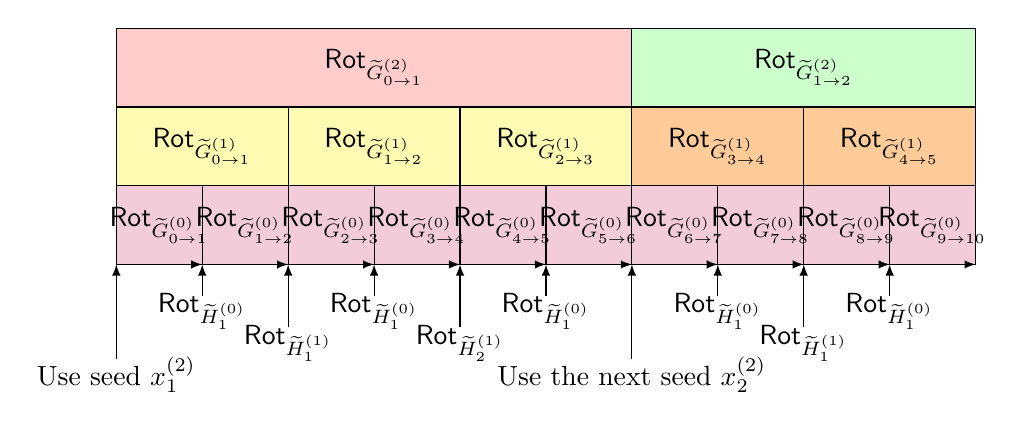
\begin{tikzpicture}

        \def\layerheight{1}
        
    

        \draw[fill=red!20] (0, 3*\layerheight) rectangle (0.6*0.9*\textwidth, 4*\layerheight);
        \node at (0.3*0.9*\textwidth, 3.5*\layerheight) {$\Rot_{\widetilde{G}^{(2)}_{0\to 1}}$};
        \draw[fill=green!20] (0.6*0.9*\textwidth, 3*\layerheight) rectangle (0.9*\textwidth, 4*\layerheight);
        \node at (0.8*0.9*\textwidth, 3.5*\layerheight) {$\Rot_{\widetilde{G}^{(2)}_{1\to 2}}$};
        

        \draw[fill=yellow!30] (0, 2*\layerheight) rectangle (0.2*0.9*\textwidth, 3*\layerheight);
        \node at (0.1*0.9*\textwidth, 2.5*\layerheight) {$\Rot_{\widetilde{G}^{(1)}_{0\to 1}}$};
        \draw[fill=yellow!30] (0.2*0.9*\textwidth, 2*\layerheight) rectangle (0.4*0.9*\textwidth, 3*\layerheight);
        \node at (0.3*0.9*\textwidth, 2.5*\layerheight) {$\Rot_{\widetilde{G}^{(1)}_{1\to 2}}$};
        \draw[fill=yellow!30] (0.4*0.9*\textwidth, 2*\layerheight) rectangle (0.6*0.9*\textwidth, 3*\layerheight);
        \node at (0.5*0.9*\textwidth, 2.5*\layerheight) {$\Rot_{\widetilde{G}^{(1)}_{2\to 3}}$};
        \draw[fill=orange!40] (0.6*0.9*\textwidth, 2*\layerheight) rectangle (0.8*0.9*\textwidth, 3*\layerheight);
        \node at (0.7*0.9*\textwidth, 2.5*\layerheight) {$\Rot_{\widetilde{G}^{(1)}_{3\to 4}}$};
        \draw[fill=orange!40] (0.8*0.9*\textwidth, 2*\layerheight) rectangle (0.9*\textwidth, 3*\layerheight);
        \node at (0.9*0.9*\textwidth, 2.5*\layerheight) {$\Rot_{\widetilde{G}^{(1)}_{4\to 5}}$};
        

        \foreach \x in {0.1, 0.2, 0.3, 0.4, 0.5, 0.6, 0.7, 0.8, 0.9, 1} {
            \draw[fill=purple!20] (\x*0.9*\textwidth-0.1*0.9*\textwidth, 1*\layerheight) rectangle (\x*0.9*\textwidth, 2*\layerheight);
            
        };
        \foreach \x in {0.1, 0.2, 0.3, 0.4, 0.5, 0.6, 0.7, 0.8, 0.9, 1} {
            \draw[->, -latex] (\x * 0.9*\textwidth-0.1*0.9*\textwidth, \layerheight) to (\x * 0.9*\textwidth, 1*\layerheight);
            }
            
        \foreach \x in {1,2,3,4,5,6,7,8,9,10} {
            \pgfmathsetmacro{\y}{\x-1}
            \node at (\x*0.9*\textwidth/10-0.05*0.9*\textwidth, 1.5*\layerheight) {$\Rot_{\widetilde{G}^{(0)}_{\pgfmathprintnumber{\y}\to \x}}$};
        }
    
        \foreach \x in {0.1, 0.3, 0.5, 0.7, 0.9} {
            \draw[->, -latex] (\x * 0.9*\textwidth, 0.6*\layerheight) to (\x * 0.9*\textwidth, 1*\layerheight);
            \node at (\x*0.9*\textwidth, 0.4*\layerheight) {$\Rot_{\widetilde{H}^{(0)}_1}$};
        }
    
        \foreach \x in {0.2,0.8} {
            \draw[->, -latex] (\x * 0.9*\textwidth, 0.2*\layerheight) to (\x * 0.9*\textwidth, 1*\layerheight);
            \node at (\x*0.9*\textwidth, 0*\layerheight) {$\Rot_{\widetilde{H}^{(1)}_1}$};
        }
    
        \foreach \x in {0.4} {
            \draw[->, -latex] (\x * 0.9*\textwidth, 0.2*\layerheight) to (\x * 0.9*\textwidth, 1*\layerheight);
            \node at (\x*0.9*\textwidth, 0*\layerheight) {$\Rot_{\widetilde{H}^{(1)}_2}$};
        }
    
         \foreach \x in {0.6} {
            \draw[->, -latex] (\x * 0.9*\textwidth, -0.2*\layerheight) to (\x * 0.9*\textwidth, 1*\layerheight);
            \node at (\x*0.9*\textwidth, -0.4*\layerheight) {Use the next seed $x^{(2)}_2$};
        }
         \foreach \x in {0.0} {
            \draw[->, -latex] (\x * 0.9*\textwidth, -0.2*\layerheight) to (\x * 0.9*\textwidth, 1*\layerheight);
            \node at (\x*0.9*\textwidth, -0.4*\layerheight) {Use seed $x^{(2)}_1$};
        }
    
        
    
        
        \end{tikzpicture}
    \caption{The figure shows our recursion process to compute $\Rot_{\widetilde{G}^{(l)}_{1 \to 2}}\left(\Rot_{\widetilde{G}^{(l)}_{0 \to 1}}\left(v_0,x^{(l)}_1\right),x^{(l)}_2\right)$ when $l = 2, n_l=2$. The indices $j_0,j_1,j_2$ are omitted.
    }
\end{figure}

Next we prove the correctness of the algorithm.


Let $ \widetilde{G}^{(0)}_{t-1\to t}$ denote the bipartite graph with two-way labeling of the input from the $(t-1)$-th layer to the $t$-th layer. We recursively define $ \widetilde{G}^{(i)}_{j_0,j_1,...,j_{i-1},t-1\to t}$ as the graph obtained by applying \cref{thm:derandomization algorithm}  to $ \widetilde{G}^{(i-1)}_{j_0,j_1,...,j_{i-2},a\to a+1}, \ldots,  \widetilde{G}^{(i-1)}_{j_0,j_1,...,j_{i-2},b-1\to b }$ where  $b=n^{(i)}_{j_{i-1},t},a=n^{(i)}_{j_{i-1},t-1}$ with the aforementioned parameters $n_i,\lambda_i,d_i,c_i$.
Let  $\widetilde{\mathbf{W}}^{(i)}_{j_0,j_1,...,j_{i-1},t\gets t-1}$ be the transition matrix of $ \widetilde{G}^{(i)}_{j_0,j_1,...,j_{i-1},t-1\to t}$.

The output of Algorithm \ref{algo:tildeG} is a weighted sum  of  $\widetilde{\mathbf{W}}^{(l)}_{j_0,j_1,...,j_{i-1}, n_l\gets n_l-1}\cdots \widetilde{\mathbf{W}}^{(l)}_{j_0,j_1,...,j_{i-1}, 1\gets 0}$, as shown in the following equation:
\begin{align*}
    &ans\\
    =&\sum_{\substack{j_0\in [W_0],j_1\in [W_1],\\\ldots,j_{l-1}\in [W_{l-1}]}}\left(\prod_{i=0}^{l-1}\sigma_{j_i}\right)\cdot \E_{x^{(l)}_1,x^{(l)}_2,\ldots,x^{(l)}_{n_l}\in [d_l]}\\
    &\left[\mathbf{1}\left[\Rot_{\widetilde{G}^{(l)}_{\substack{j_0,j_1,\ldots,j_{l-1}\\ ,n_l-1 \to n_l}}}\left(\cdots\Rot_{\widetilde{G}^{(l)}_{\substack{j_0,j_1,\cdots,j_{l-1}\\ ,1 \to 2}}}\left(\Rot_{\widetilde{G}^{(l)}_{\substack{j_0,j_1,\cdots,j_{l-1}\\ ,0 \to 1}}}\left(v_0,x^{(l)}_1\right),x^{(l)}_2\right)\ldots,x^{(l)}_{n_l}\right)=v_{end}\right]\right]\\
    =&\sum_{\substack{j_0\in [W_0],j_1\in [W_1],\\\ldots,j_{l-1}\in [W_{l-1}]}}\left(\prod_{i=0}^{l-1}\sigma_{j_i}\right)\cdot 
    \left[\widetilde{\mathbf{W}}^{(l)}_{j_0,j_1,...,j_{i-1},n_l\gets n_l-1}\cdots \widetilde{\mathbf{W}}^{(l)}_{j_0,j_1,...,j_{i-1},1\gets 0}
\right]_{v_0,v_{end}}.
\end{align*}


By \cref{lem:sv approximation algorithm}, for any $i\in [l],j_0,j_1,...,j_{i-1}\in [W_0],[W_1],...,[W_{i-1}]$, letting $b=n^{(i)}_{j_{i-1},t},a=n^{(i)}_{j_{i-1},t-1}$, we have the following approximation.
\begin{align*}
    \widetilde{\mathbf{W}}^{(i)}_{j_0,j_1,...,j_{i-1},t\gets t-1} \sv_{\tau_{i-1}}\widetilde{\mathbf{W}}^{(i-1)}_{j_0,j_1,...,j_{i-2},b\gets b-1}\widetilde{\mathbf{W}}^{(i-1)}_{j_0,j_1,...,j_{i-2},b-1\gets b-2}\ldots \widetilde{\mathbf{W}}^{(i-1)}_{j_0,j_1,...,j_{i-2},a\gets a+1}.
\end{align*}


These matrices satisfy the condition of \cref{lem:derandErrorRedPoly}. By the construction of the $\{n^{(i)}_{j,t}\}$ and $\{\sigma_{j}\}$, we have that for each $i\in {0,1,\ldots,l-1}$ and each $j_0,j_1,\ldots,j_{i-1}$,
\begin{align*}
    \left|\left[\widetilde{\mathbf{W}}^{(i)}_{\substack{j_0,...,j_{i-1}\\n_i\gets n_i-1}} \cdots \widetilde{\mathbf{W}}^{(i)}_{\substack{j_0,...,j_{i-1}\\1\gets 0}}\right]_{v_0,v_{end}}-\sum_{j_i\in [W_i]}\left[\sigma_{j_i}\cdot \widetilde{\mathbf{W}}^{(i+1)}_{\substack{j_0,...,j_{i}\\n_{i+1}\gets n_{i+1}-1}}\cdots \widetilde{\mathbf{W}}^{(i+1)}_{\substack{j_0,...,j_{i}\\1\gets 0}}\right]_{v_0,v_{end}}\right|\leq \alpha_i.
\end{align*}




By summing over all the errors, we have the following:
\begin{align*}
    &\left|ans-\left[\widetilde{\mathbf{W}}^{(0)}_{n_0\gets n_0-1} \cdots \widetilde{\mathbf{W}}^{(0)}_{1\gets 0}\right]_{v_0,v_{end}}\right|\\
    =& \left|\sum_{i=0}^{l-1}\sum_{\substack{j_0\in [W_0],j_1\in [W_1],\\\ldots,j_{i-1}\in [W_{i-1}]}}\left(\prod_{k=0}^{i-1}\sigma_{j_k}\right)\right.\\
    &\left.\cdot\left(\left[\widetilde{\mathbf{W}}^{(i)}_{\substack{j_0,...,j_{i-1}\\n_i\gets n_i-1}} \cdots \widetilde{\mathbf{W}}^{(i)}_{\substack{j_0,...,j_{i-1}\\1\gets 0}}\right]_{v_0,v_{end}}-\sum_{j_i\in [W_i]}\left[\sigma_{j_i}\cdot \widetilde{\mathbf{W}}^{(i+1)}_{\substack{j_0,...,j_{i}\\n_{i+1}\gets n_{i+1}-1}}\cdots \widetilde{\mathbf{W}}^{(i+1)}_{\substack{j_0,...,j_{i}\\1\gets 0}}\right]_{v_0,v_{end}}\right)\right|
    \\
    \leq& \sum_{i=0}^{l-1}\sum_{\substack{j_0\in [W_0],j_1\in [W_1],\\\ldots,j_{i-1}\in [W_{i-1}]}}\alpha_i\\
    \leq& \alpha_0+W_0\cdot \alpha_1+\ldots+W_0\cdot W_1\cdots W_{l-1}\cdot \alpha_l.
\end{align*}


By our parameters, this entry-wise error is at most $\varepsilon/w$. Therefore, the total error is at most $\varepsilon$ when the accept node set is an arbitrary subset of $V_n=[w]$.

Then we prove the space complexity of the algorithm. Similar to the proof of \cref{lem:permutation-reduction-main}, $d_l=O(\log n(\log\log n+\sqrt{\log(w/\varepsilon)})+\log(w/\varepsilon))$, which is exactly the seed length in that proof. The algorithm shall store $ans$, $j_i,n_i$ for each $i\in [l-1]$ and $x^{(l)}$, which costs no more than $O(s+\log n(\log\log n+\sqrt{\log(w/\varepsilon)})+\log(w/\varepsilon))$ space. Calculating a two-way labeling and computing $\Rot_{G^{(0)}_{t\gets t-1}}$ cost $O(s+\log (nw))$ space. The computation of $\Rot_{H^{(i)}_t}$ costs $O(|x^{(i)}|)$ space according to \cref{lem:space-efficient expanders}.
 Therefore, the total space complexity is $O(s+\log n(\log\log n+\sqrt{\log(w/\varepsilon)})+\log(w/\varepsilon))$.
    



\end{proof}


























\bibliographystyle{alpha}
\bibliography{ref}
\appendix
\section{A proof for \cref{thm:NZonelayer}}\label{sec:NZproof}

We reprove the lemma for completeness. 

\begin{definition}[total variation]
Let ${A}$ and ${B}$ be two random variables defined on a common probability space $X$. The total variation distance between ${A}$ and ${B}$ is defined as
\begin{align*}
    d_{TV}({A},{B})=\frac{1}{2}\sum_{x\in X}\left|\Pr[{A}=x]-\Pr[{B}=x]\right|.
\end{align*}
\end{definition}

\begin{definition}[Min-Entropy]
    Let ${X}$ be a random variable. The min-entropy of ${X}$ is defined as
    \begin{align*}
        H_{\infty}({X})=-\log_2\left(\max_{x\in X}\Pr[{X}=x]\right).
    \end{align*}
\end{definition}

\begin{definition}[Conditional Min-Entropy \cite{vadhanPseudorandomness2012} Problem 6.7]
    Let ${X}$ and ${A}$ be two random variables. The conditional min-entropy of ${X}$ given ${Y}$ is defined as
    \begin{align*}
        \tilde{H}_{\infty}({X}|{Y})=-\log_2\left(\underset{y\in Y}{\E}\sup_{x\in X}\Pr[{X}=x|{Y}=y]\right).
    \end{align*}
\end{definition}



We need the following lemmas.

\begin{lemma}[Chain rule of Conditional Min-Entropy \cite{vadhanPseudorandomness2012} Problem 6.7]\label{lem:chainrule}
    If $|\text{supp}(A)|\leq 2^s$, then $\widetilde{H}_{\infty}(X|A)\geq H_{\infty}(X)-s$.
\end{lemma}

\begin{lemma}[Problem 6.8 of \cite{vadhanPseudorandomness2012}]\label{lem:extractor for conditional min-entropy}
    Let $Ext:\{0,1\}^n\times \{0,1\}^d\to \{0,1\}^m$ be a $(k,\varepsilon)$-extractor. If $\tilde{H}_{\infty}({X}|{A})\geq k$, then 
    $$
    d_{TV}\left((Ext({X},U_d),A),(U_m,A)\right)\leq 3\varepsilon.
    $$
    (Here $U_m$ and $U_d$ are independent uniform random variables of length $m$ and $d$ respectively.)
\end{lemma}

\begin{lemma}[Data Processing Inequality]
    Let $X,Y$ be two random variables in the same probability space. Let $A$ be a random variable that is independent of both $X$ and $Y$. Let $f$ be a function. Then 
    \begin{align*}
        d_{TV}(f(X,A),f(Y,A))\leq d_{TV}(X,Y).
    \end{align*}
\end{lemma}


Now we can prove the lemma.
\begin{lemma}[\cref{thm:NZonelayer} restated]
    Let $s\geq \log w$. Assume there exists a $(2s, \frac{\varepsilon}{3n})$-extractor $\Ext:\{0,1\}^{3s}\times \{0,1\}^{d}\to \{0,1\}^{s}$.  Let $X$ and $Y_1,\ldots,Y_n$ be independent uniform random variables. Then the following construction
    \begin{align*}
        \NZ(X,Y)=\Ext(X,Y_1), \ldots, \Ext(X,Y_n)
    \end{align*}
    fools any $f\in \mathcal{B}_{(n,s,w)}$ with error at most $\varepsilon$.
\end{lemma}



\begin{proof}
    Let $f\in \mathcal{B}_{(n,s,w)}$. Let $X$ and $Y_1,\ldots,Y_n$ be independent uniform random variables. We use a hybrid argument.  Define $U_i$ to be independent uniform random variables of length $s$ for each $i\in [n]$. Define $Z_i=\Ext(X,Y_i)$ for each $i\in [n]$. Define $R_i$ to be the random variable over $V_i$, which represents the distribution of the state of $f$ on input $U_1,\ldots,U_i$. Define $\widetilde{R}_i$ to be the random variable over $V_i$ which represents the distribution of the state of $f$ on input $Z_1,\ldots,Z_i$. We will show that $d_{TV}(R_i,\widetilde{R}_i)\leq \frac{i\cdot \varepsilon}{n}$ for all $i\in [n]$.

    The base case $i=0$ is trivial, as both $R_0$ and $\widetilde{R}_0$ represent the initial state of $f$. Assume the statement holds for $i-1$. 
    For the case $i$, notice that $|\text{supp}(\widetilde{R}_{i-1})|\leq w\leq 2^s$. By the chain rule \cref{lem:chainrule}, 
    $$\tilde{H}_{\infty}(X|\widetilde{R}_{i-1})\geq 2s.$$ 
    Therefore \cref{lem:extractor for conditional min-entropy} implies 
    $$
    d_{TV}((Z_i,\widetilde{R}_{i-1}),(U_i,\widetilde{R}_{i-1}))\leq \frac{\varepsilon}{n}.
    $$
    By the data processing inequality, we have
    $$
    d_{TV}((U_i,\widetilde{R}_{i-1}),(U_i,R_{i-1}))\leq d_{TV}(\widetilde{R}_{i-1},R_{i-1})\leq \frac{(i-1)\varepsilon}{n}.
    $$
    Using the triangle inequality, we have
    $$
    d_{TV}((Z_i,\widetilde{R}_{i-1}),(U_i,R_{i-1}))\leq \frac{i\varepsilon}{n}.
    $$
    Denote the transition function of $f$ from $V_{i-1}$ to $V_i$ as $T_i$. Then $\widetilde{R}_i=T_i(Z_i,\widetilde{R}_{i-1})$ and $R_i=T_i(U_i,R_{i-1})$. Using the data processing inequality again, we have
    $$
    d_{TV}(R_i,\widetilde{R}_i)\leq d_{TV}((U_i,R_{i-1}),(Z_i,\widetilde{R}_{i-1}))\leq \frac{i\varepsilon}{n}.
    $$
    Therefore, $d_{TV}(R_n,\widetilde{R}_n)\leq \varepsilon$ and the lemma is proved.
\end{proof}

\section{A proof for \cref{thm:richardson iteration}}\label{appendix:iterationproof}
We prove \cref{thm:richardson iteration} using the Richardson Iteration for completeness. The Richardson iteration is a method to obtain a finer approximation of $L^{-1}$ from a coarse approximation $B$ of $L^{-1}$ and the invertible matrix $L$ itself. 

\begin{lemma}
    Let $L\in \mathbb{R}^{m\times m}$ be an invertible matrix and $B\in \mathbb{R}^{m\times m}$ such that $\|B-L^{-1}\|\leq \varepsilon_0$ for a submultiplicative norm $\|\cdot\|$. For any non-negative integer $k$, define
    \begin{align*}
        R(B,L,k)=\sum_{i=0}^{k}(I-BL)^{i}B
    \end{align*}
    Then $\|L^{-1}-R(B,L,k)\|\leq \|L^{-1}\|\cdot\|L\|^{k+1}\cdot \varepsilon_0^{k+1}$.
\end{lemma}

\begin{proof}
    \begin{align*}
        \|L^{-1}-R(B,L,k)\|&=\left\lVert \left(I-\sum_{i=0}^{k}(I-BL)^{i}BL\right)L^{-1}\right\rVert\\
        &=\left\lVert(I-BL)^{k+1}L^{-1}\right\rVert\\ 
        &\leq \left\lVert I-BL\right\rVert^{k+1}\cdot \left\lVert L^{-1}\right\rVert\\
        &\leq \left\lVert L^{-1}\right\rVert\cdot \left\lVert L\right\rVert^{k+1}\cdot \varepsilon_0^{k+1}
    \end{align*}
\end{proof}


\begin{theorem}[\cref{thm:richardson iteration} restated]
    Let $\{A_i\}_{i=1}^n\subset \mathbb{R}^{w\times w}$ be a sequence of matrices. Let $\{B_{i,j}\}_{i,j=0}^n \subset \mathbb{R}^{w\times w}$ be a family of matrices such that for every $i+1< j$, $\|B_{i,j}-A_{i+1}\ldots A_j\|\leq \varepsilon/(n+1)^2$ for some submultiplicative norm $\|\cdot\|$, $\|A_i\|\leq 1$ for all $i$ and also $B_{i-1,i}=A_i$ for all $i$. Then for any odd $k\in \mathbb{N}$, there exists a $K=(8n)^{k+1}$, a set of indices $\{n_{i,j}\}_{i\in [K], j\in [k]}$ with $0\leq n_{i,1}\leq \ldots\leq n_{i,k}= n$, and  signs $\sigma_i\in\{-1,0,1\} , i\in [K]$ such that (We set $B_{i,i}=I$ for all $i$):

    \begin{align*}
        \left\lVert A-\sum_{i\in [K]}\sigma_i\cdot B_{0,n_{i,1}}B_{n_{i,1},n_{i,2}}\ldots B_{n_{i,k-1},n_{i,k}}\right\rVert\leq \varepsilon^{(k+1)/2}\cdot(n+1).
    \end{align*}

    
\end{theorem}
\begin{proof}
    


Define $L\in \mathbb{R}^{(n+1)w\times (n+1)w}$ and $B\in \mathbb{R}^{(n+1)w\times (n+1)w}$ as follows:

\begin{align*}
    L&=
    \begin{pmatrix}
        I & 0 & 0 & \ldots & 0 & 0\\
        -A_1 & I & 0 & \ldots & 0 & 0\\
        0 & -A_2 & I & \ldots & 0 & 0\\
        \vdots & \vdots & \vdots & \ddots & \vdots & \vdots\\
        0 & 0 & 0 & \ldots & -A_{n} & I\\
    \end{pmatrix},
    B=
    \begin{pmatrix}
        I & 0 & 0 & \ldots & 0 & 0\\
        B_{0,1} & I & 0 & \ldots & 0 & 0\\
        B_{0,2} & B_{1,2} & I & \ldots & 0 & 0\\
        \vdots & \vdots & \vdots & \ddots & \vdots & \vdots\\
        B_{0,n} & B_{1,n} & B_{2,n} & \ldots & B_{n-1,n} & I\\
    \end{pmatrix}
\end{align*}
This means that 
\begin{align*}
    L^{-1}=
    \begin{pmatrix}
        I & 0 & 0 & \ldots & 0 & 0\\
        A_1 & I & 0 & \ldots & 0 & 0\\
        A_1A_2 & A_2 & I & \ldots & 0 & 0\\
        \vdots & \vdots & \vdots & \ddots & \vdots & \vdots\\
        A_1A_2\ldots A_{n} & A_2\ldots A_{n} & A_3\ldots A_{n} & \ldots & A_{n} & I\\
    \end{pmatrix}
\end{align*}

By assumption, there exists a submultiplicative norm $\|\cdot\|$ on $\mathbb{R}^{w\times w}$. We induce a submultiplicative norm on $\|\cdot\|_A$ on $\mathbb{R}^{(n+1)w\times (n+1)w}$: Let $M=(M_{i,j})_{i,j=1}^{n+1}\in \mathbb{R}^{(n+1)w\times (n+1)w}$, where each $M_{i,j}\in \mathbb{R}^{w\times w}$. Define $\|M\|_A=\max_{j\in [n+1]}\sum_{i=1}^{n+1}\|M_{i,j}\|$. It is easy to verify that $\|\cdot\|_A$ is a submultiplicative norm, and $\|M\|_A=\|M\|_1$ when $w=1$.

Beacuse $\|B_{i,j}-A_{i+1}\ldots A_j\|\leq \varepsilon/(n+1)^2$ for all $i+1< j$, we have $\|B-L^{-1}\|_A\leq \varepsilon/(n+1)$. 
Also, Because $\|A_i\|\leq 1$ for all $i$, we have $\|L\|_A\leq n+1$ and $\|L^{-1}\|_A\leq n+1$.

Define $M=R(B,L,(k-1)/2)$, then 
\begin{align*}
    \|L^{-1}-M\|_A\leq \|L^{-1}\|_A\cdot\|L\|_A^{\frac{k+1}{2}}\cdot \left(\frac{\varepsilon}{n+1}\right)^{\frac{k+1}{2}}\leq \varepsilon^{(k+1)/2}\cdot(n+1).
\end{align*}

Expand $M=(M_{i,j})_{i,j=1}^{n+1}$, where each $M_{i,j}\in \mathbb{R}^{w\times w}$. We foucus on $M_{1,n+1}$, which is a $w\times w$ matrix and $\|M_{1,n+1}-A_1A_2\ldots A_n\|\leq \|L^{-1}-M\|_A\leq \varepsilon^{(k+1)/2}\cdot(n+1)$.

To express $M_{1,n+1}$, we define
\begin{align*}
    \Delta_{i,j}=\begin{cases}
        B_{i,j-1}A_j-B_{i,j} &  i<j,\\
        0 & i\geq j.
    \end{cases}
\end{align*}

Then we have
\begin{align*}
    M_{1,n+1}=B_{0,n}+\sum_{j=1}^{(k-1)/2}\sum_{0<r_1<\cdots<r_j<n}\Delta_{0,r_1}\Delta_{r_1,r_2}\cdots \Delta_{r_{j-1},r_j}B_{r_j,n}.
\end{align*}

Defining $M^{(0)}_{i,j}=B_{i,j-1}A_j=B_{i,j-1}B_{j-1,j}$ and $M^{(1)}_{i,j}=B_{i,j}$, we have
\begin{align*}
    M_{1,n+1}=B_{0,n}+\sum_{j=1}^{(k-1)/2}\sum_{0<r_1<\cdots<r_j<n}\sum_{t_1,\ldots,t_j\in \{0,1\}}(-1)^{t_1+\cdots+t_j} M^{(t_1)}_{0,r_1}M^{(t_2)}_{r_1,r_2}\ldots M^{(t_j)}_{r_j,n}.
\end{align*}

Encoding $j,r_1,\ldots,r_j,t_1,\ldots,t_j$ into a single index $i\in[K]$, rewrite $M^{(t_1)}_{0,r_1}M^{(t_2)}_{r_1,r_2}\ldots M^{(t_j)}_{r_j,n}$ as $B_{0,n_{i,1}}B_{n_{i,1},n_{i,2}}\ldots B_{n_{i,k-1},n_{i,k}}$ for some $n_{i,1}\leq \ldots\leq n_{i,k}=n$, define $\sigma_i=(-1)^{t_1+\ldots+t_j}$, we have the desired result.

Finally, we bound $K$ by $\frac{k-1}{2}\cdot (n+1)^{(k-1)/2}\cdot 2^{(k-1)/2}\leq (8n)^{k+1}$.



\end{proof}


\section{A Proof for \cref{lem:sampler for small error}}\label{append:smallererr}


In this section we provide a proof for \cref{lem:sampler for small error}, which is similar to that of \cite{hozaBetterPseudodistributionsDerandomization2021}. We start by sampling a random matrix using a sampler, using a union bound.

\begin{lemma}\label{lem:matrix sampler}
    Let $\Samp: \{0, 1\}^p \times \{0, 1\}^r \rightarrow \{0, 1\}^q$ be a $(\alpha,\gamma)$-averaging sampler.  Then for every matrix valued function $f:\{0,1\}^q\to \mathbb{R}^{w\times w}$ such that $\|f\|_{1}\leq C$, we have:
    \begin{align*}
        \Pr_{x \in \{0,1\}^r }\left[\left\|2^{-p}\sum_{y\in \{0,1\}^p}  f(\Samp(x,y)) - \E [f] \right\|_{1} \ge C \alpha w \right]\leq w^2\gamma.
    \end{align*}
\end{lemma}

\begin{proof}
    \begin{align*}
        &\Pr_{x \in \{0,1\}^r }\left[\left\|2^{-p}\sum_{y\in \{0,1\}^p}  f(\Samp(x,y)) - \E [f] \right\|_{1} \ge C \alpha w \right]\\
        =&\Pr_{x \in \{0,1\}^r }\exists_{i\in [w]}\left[\sum_{j\in [w]} \left[2^{-p}\sum_{y\in \{0,1\}^p}  f(\Samp(x,y))_{i,j} - \E [f]_{i,j} \right] \ge C \alpha w \right]\\
        \leq&\Pr_{x \in \{0,1\}^r }\exists_{i\in [w],j\in [w]}\left[\left|2^{-p}\sum_{y\in \{0,1\}^p}  f(\Samp(x,y))_{i,j} - \E [f]_{i,j} \right| \ge C \alpha \right]\\
        \leq&\sum_{i\in [w],j\in [w]}\Pr_{x \in \{0,1\}^r }\left[\left|C^{-1}2^{-p}\sum_{y\in \{0,1\}^p}  f(\Samp(x,y))_{i,j} - C^{-1}\E [f]_{i,j} \right| \ge \alpha \right]\\
        \leq& w^2 \gamma.
    \end{align*}
\end{proof}



\begin{lemma}[\cref{lem:sampler for small error} restated]
    For all $n,s,w$, assume there exists a $W$-bounded $1/(2w\cdot (n+1)^2)$-WPRG $(G_0,w_0)$  for $\mathcal{B}_{(n,s,w)}$ with seed length $d$, and a $(\alpha,\gamma)$-averaging sampler $\Samp:\{0,1\}^r \times \{0,1\}^p\to \{0,1\}^d$ with $\alpha,\gamma$ as defined above. Then there exists a $\varepsilon$-WPRG for $\mathcal{B}_{(n,s,w)}$ with seed length $r+kp$ and weight $W^{log(n/\varepsilon)/\log (nw)}\cdot \poly(nw/\varepsilon)$.
\end{lemma}

\begin{proof}
    Take any $f\in \mathcal{B}_{(n,s,w)}$. Let $A_i=\E f^{[i-1,i]}(G_0(U))$ for $i\in [n]$. Define $B_{i,j}=\frac{1}{2^p}\sum_{z\in \{0,1\}^d} w_0(z)\cdot f^{[i,j]}(G(z))$. For any $x\in \{0,1\}^r$, we define $B^x_{i,j}=\frac{1}{2^p}\sum_{y\in \{0,1\}^p} w_0(\Samp(x,y))\cdot f^{[i,j]}((G(\Samp(x,y)))_{j-i})$.

    We call a seed $x$ to be `good' iff for all $i,j\in [n]$, $\|B_{i,j}-B^x_{i,j}\|_1\leq 1/(2w\cdot (n+1))$. Otherwise, we call $x$ to be `bad'. 
    
    Since $w_0$ is $W$-bounded, $\|w_0(z)\cdot f^{[i,j]}(G(z))\|_1$ is at most $W$. Note that $W\alpha w\leq 1/(2w\cdot (n+1)^2)$. By Lemma~\ref{lem:matrix sampler}, for any $i,j\in [n]$, 
    \begin{align*}
        \Pr_{x\in \{0,1\}^r}[\|B_{i,j}-B^x_{i,j}\|_1>1/(2w\cdot (n+1))]\leq w^2\gamma=\varepsilon/(2(2n)^k\cdot W^{k}).
    \end{align*}

    By a union bound, the probability $\Pr_{x\in \{0,1\}^r}[x \text{ is bad}]$ is at most $\varepsilon/(2(2n)^k\cdot W^{k})$. 

    For a good seed $x$, we have $\|A_i\ldots A_j-B^x_{i,j}\|_1\leq \|A_i\ldots A_j-B_{i,j}\|_1+\|B_{i,j}-B^x_{i,j}\|_1\leq 1/(w\cdot (n+1)^2)$. By Theorem~\ref{thm:richardson iteration}, 
    we have:
    \begin{align*}
        \left\|A_1\cdots A_n-\sum_{i=1}^{k}\sigma_i B^x_{0,i_1}B^x_{i_1,i_2}\ldots B^x_{i_{k-1},i_k}\right\|_1
        \leq ((n+1)w)^{-k}\cdot (n+1)\leq \varepsilon/2.
    \end{align*}

    \iffalse
    Using a similar argument as in Lemma~\ref{lem:framework}, we have the following inequality:
    \begin{align*}
        \left|\E f-\frac{1}{K\cdot 2^{kq}}\sum_{i=0}^{k}\sum_{y_1,\ldots,y_{k}\in \{0,1\}^p}w(x,y_1,\ldots,y_{k},i)f(G(x,y_1,\ldots,y_{k}))\right|\leq \varepsilon/2.
    \end{align*}
    \fi

    For a bad seed, we can upper-bound $\|B^x_{i,j}\|_1$ by $K$. Therefore, we have:
    \begin{align*}
         \left\|A_1\cdots A_n-\sum_{i=1}^{K}\sigma_i B^x_{0,i_1}B^x_{i_1,i_2}\ldots B^x_{i_{k-1},i_k}\right\|_1
        \leq 1+K\cdot W^k
    \end{align*}
    
    Combining the two cases, we have the following inequality:
    \begin{align*}
        &\left|\E f- \frac{1}{K\cdot 2^{kp+r}}\sum_{x\in \{0,1\}^r}\sum_{y_1,\ldots,y_{k}\in \{0,1\}^p}w(x,y_1,\ldots,y_{k},i)f(G(x,y_1,\ldots,y_{k}))\right|\\
        \leq&\left\|A_1\cdots A_n-\frac{1}{2^r}\sum_{x\in \{0,1\}^r}\sum_{i=1}^{K}\sigma_i B^x_{0,i_1}B^x_{i_1,i_2}\ldots B^x_{i_{k-1},i_k}\right\|_1\\
        \leq&\frac{1}{2^r}\sum_{\substack{x\in \{0,1\}^r \\ x \text{ is bad}}}\left\|A_1\cdots A_n-\sum_{i=1}^{K}\sigma_i B^x_{0,i_1}B^x_{i_1,i_2}\ldots B^x_{i_{k-1},i_k}\right\|_1\\
        &+\frac{1}{2^r}\sum_{\substack{x\in \{0,1\}^r \\ x \text{ is good}}}\left\|A_1\cdots A_n-\sum_{i=1}^{K}\sigma_i B^x_{0,i_1}B^x_{i_1,i_2}\ldots B^x_{i_{k-1},i_k}\right\|_1\\
        \leq&\varepsilon/2+(1+K\cdot W^k)\cdot\gamma\\
        \leq&\varepsilon.
    \end{align*}

    The lemma follows.
\end{proof}



\section{Transforming regular ROBPs to permutation ROBPs in the binary edge label setting}\label{sec:binaryRegulartoPerm}

\begin{lemma}
    There is an algorithm which on inputting a regular ROBP $P$ with length $n$ width $w$ and binary edge labels, outputs a permutation ROBP $P'$ with length $n$ width $w$ and binary edge labels.
    The algorithm has workspace $O(\log (nw))$.
\end{lemma}
\begin{proof}
$P'$ has the same vertex set as that of $P$.
The algorithm transforms each layer $i $ of $P$ in the order $i = 0, 1, 2, \ldots, n$.
For layer $i$, consider the subgraph $S$ between $V_i$ and $V_{i+1}$. The algorithm handles each node $v \in V_i$ in order.
For each $v \in V_i$, if it is not reachable by any previous node of $V_i$ in $S$, which can be done in logspace, then it does the following traverse in $S$. Starting from $v$, choose an edge with label $0$, and then go to the corresponding neighbor. For each next neighbor $u$ visited, use $\ell$ to record the label of the edge $e$ it just traverses to this neighbor. If the other adjacent edge $e'$ the neighbor has a label $\ell' = \ell$ then flip its label.
Then traverse through this edge $e'$ to go to the next neighbor. 
Go on doing this until it reaches $v$ again.

Notice that starting from $v$ we can visit every node of $V_i \cup V_{i+1}$ that is reachable from $v$ in the above traverse. Because for each next neighbor $u$, it can only be either $v$ or a node which is not visited before in this traverse, since except $v$, every node visited already has both adjacent edges visited, and the traverse only visits edge that is not visited before.

Also after the traverse, every node reachable from $v$ in $V_{i+1}$, because of the flipping, can have different labels for the two adjacent edges. So the induced graph by these nodes reachable, becomes a permutation.
Notice that for each next $v \in V_i$, we only do the traverse when it is not reachable from previous nodes in $V_i$. So each edge will be visited and may be flipped only once.

After we went through every $v \in V_i$, all nodes of $V_{i+1}$ in $S$ are reached. So we have a permutation.

\end{proof}


\section{Proof sketch for \cref{lem:sv-fool}}\label{sec:sv-fool sketch}

Though not explicitly mentioned, the analysis of the INW generator in appendix B of \cite{chenWeightedPseudorandomGenerators2023} works for large alphabet ROBPs. Here we slightly modifies their proof to make it explicitly works.

We start with the definition of the INW generator. Some notions are defined in the preliminaries of \cref{sec:derand regular} 

\begin{definition}[INW generator for large alphabets]
Let $n,c,d$ be powers of two. For each $t\in [\log n]$, let $H_t$ be a $c$-regular bigraph $H_t=([d\cdot c^{t-1}],[d\cdot c^t],E_{H_t})$, with a one-way label. Relative to the family $(H_t)_{t\in [\log n]}$, we recursively define the INW generator as follows:

Define $\INW_0:\{0,1\}^{\log d}\to \{0,1\}^{\log d}$ as the trivial PRG. For each $t\in [\log n]$, having defined $\INW_{t-1}:\{0,1\}^{d+(t-1)\log c}\to \{0,1\}^{\log d\cdot 2^{t-1}}$, we define $\INW_t:\{0,1\}^{d+t\log c}\to \{0,1\}^{\log d\cdot 2^t}$ as $\INW_t(x,y)=\INW_{t-1}(x),\INW_{t-1}(H_t[x,y])$. Here the comma denotes concatenation.
    
\end{definition}

The INW generator relates to the derandomized product of permutation ROBPs, since they have consistent one-way labelings.

\begin{definition}[consistent consistent one-way labelings]
    Let $G=(U,V,E)$ be a $d$-regular bigraph. A consistent one-way labeling of $G$ is a one-way labeling of $G$ such that for every $v\in V$, the labels of the incoming edges of $v$ are distinct, i.e., the $G[v,i]=G[u,i]$ implies $u=v$. In this case, we can extend the labeling to a two-way labelings:
    \begin{align*}
        \Rot_G(u,i)=(G[u,i],i),
    \end{align*}
    i.e., the incoming label and the outgoing label of an edge $(u,v)$ are the same.
\end{definition}


\begin{lemma}[Derandomized Product with consistent consistent one-way labelings,\cite{rozenmanDerandomizedSquaringGraphs2005}]
    Let $G_1=(U,V,E_1)$ and $G_2=(V,W,E_2)$ be two $d$-regular bigraphs with consistent one-way labelings. Let $H$ be a $x$-regular bigraph with one-way labeling. Then $G_1\ds_H G_2$ has a consistent one-way labeling.
\end{lemma}

Let $f$ be a permutation ROBP in $\mathcal{P}_{(n,s)}$. Then $f$ is also a regular ROBP with a consistent labeling. It can be sv-approximated with the method of \cref{lem:sv approximation algorithm}. Furthermore, the method corresponds to fooling $f$ with the INW generator.

\begin{lemma}[equivariance between INW generator and \cref{lem:sv approximation algorithm}]
    Let $f$ be a permutation ROBP in $\reduct{P}_{(n,s)}$. Let $t\in [\log n]$, $(j,j+2^t)\in E_{SC_n}$ and $\widetilde{G}_{j,j+2^t}$ be the $(d\cdot c^t)$-regular bigraph with two-way labeling as defined in \cref{lem:sv approximation algorithm}. Then for any $u\in V^{j}$ and $x\in \{0,1\}^{d+t\log c}$, we have
    $$
    \exists x',\widetilde{G}_{j,j+2^t}[u,x]=[v,x'] \Leftrightarrow \left[f^{[j,j+2^t]}(\INW(x))\right]_{u,x}=v,
    $$
\end{lemma}

\begin{proof}
    The proof is by induction on $t$. For the base case $t=0$, both sides mean $u$ has an outgoing edge labeled $x$ going to $v$.
     Assume the statement holds for $t-1$. Recall that 
    \[
\widetilde{G}_{ j \to j+2^t} = \widetilde{G}_{ j \to j+2^{t-1}} \ds_{H_t} \widetilde{G}_{j+2^{t-1}\to j+2^t}, \forall t \ge 1,
\] 
    Then for $t$, the left side can be computed as follows (where $x=(z,y)$):
    \begin{align*}
        &(w,z)=\Rot_{\widetilde{G}_{j,j+2^{t-1}}}(u,z),\\
        &(z',y')=\Rot_{H_t}(z,y),\\
        &(v,w)=\Rot_{\widetilde{G}_{j+2^{t-1},j+2^t}}(z',y').
    \end{align*}
    Where the right side can be computed as follows:
    \begin{align*}
        &f^{[j,j+2^{t-1}]}(\INW_{t-1}(z))=w,\\
        &H_t[z,y]=z',\\
        &f^{[j+2^{t-1},j+2^t]}(\INW_{t-1}(z'))=v.
    \end{align*}
    The induction hypothesis implies that the two sides are equivalent.
\end{proof}


Finally, we can prove the lemma.

\begin{lemma}[\cref{lem:sv-fool} restated]
    For all $s,n,\varepsilon$ there exists a PRG (actually the INW generator) that fools $\mathcal{P}_{(n,s)}$ with $\varepsilon$-sv-error. The seed length is
    \begin{align*}
        s+O(\log n(\log\log n+\log(1/\varepsilon))).
    \end{align*} 
\end{lemma}
\begin{proof}
    Let $\lambda=\min\{\varepsilon/(11\log n),1/6(\log^2 n)\}$. Let $d=2^s$ and for each $t\in [\log n]$, let $H_t$ be a $c$-regular  expanders with $\lambda(H_t)\leq \lambda$ from \cref{lem:space-efficient expanders}. Let $\{\INW_t\}_{t\in [\log n]}$ be the INW generator from the definition. Let $\INW=\INW_{\log n}$. Then $\INW$ is a PRG with seed lengths
    $$ \log d+t\cdot \log c=s+O(\log n(\log\log n+\log(1/\varepsilon))).$$

    For any $f\in \mathcal{P}_{(n,s)}$, the derandomized product of $f$ coincides with the the output of $f\circ INW$, i.e. $\widetilde{\mathbf{W}}_{n\gets 0}=E_X f^{[0,n]}(\INW(X))$. Since $\widetilde{\mathbf{W}}_{n\gets 0}\sv_{11\lambda\log n} \widetilde{\mathbf{W}}_{n\gets n-1}\cdots \widetilde{\mathbf{W}}_{1\gets 0}$ by  \cref{lem:sv approximation algorithm}, $INW$ fools $f$ with $\varepsilon$-sv-error.
\end{proof}

\end{document}


\typeout{get arXiv to do 4 passes: Label(s) may have changed. Rerun}
